%%%%%%%%%%%%%%%%%%%%%%%%%%%%%%%%%%%%%%%%%%%%%%%%%%%%%%%%%%%%%%%%%%% 
%                                                                 %
%                            ROOT FILE                            %
%                                                                 %
%%%%%%%%%%%%%%%%%%%%%%%%%%%%%%%%%%%%%%%%%%%%%%%%%%%%%%%%%%%%%%%%%%% 
%
%  Run LaTeX or pdfLaTeX on this file to produce your thesis.
%  To produce the abstract title page followed by the abstract,
%  see the file abstitle-phd.tex or abstitle-mas.tex.
%
%%%%%%%%%%%%%%%%%%%%%%%%%%%%%%%%%%%%%%%%%%%%%%%%%%%%%%%%%%%%%%%%%%%
\documentclass[chap]{rpi_thesis}  
% Use the first command below if you want captions over 1 line indented. A side
% effect of this is to remove the use of bold for captions (thesis default).
% To restore bold, also include the second line below.
\usepackage[hang]{caption}      % to indent subsequent lines of captions
\renewcommand{\captionfont}{\bfseries} % bold caption (needed with caption 
                                       % package to restore boldface.)                       

\captionsetup[algorithm]{labelsep=colon}

\usepackage{graphics}
\usepackage{graphicx}
\usepackage{url} 
\urlstyle{rm}

% For algorithms
\usepackage{algpseudocode}
\usepackage[chapter]{algorithm}

\renewcommand{\algorithmicrequire}{\textbf{Input:}}
\renewcommand{\algorithmicensure}{\textbf{Output:}}

% For code
\usepackage{listings}
\renewcommand*{\lstlistlistingname}{LIST OF LISTINGS}

% For equations 
\usepackage{amsmath}
\usepackage{amsfonts}
\usepackage{amssymb}

\renewcommand{\vec}[1]{\mathbf{#1}}

% For rotating in the tables
\usepackage{rotating} 
\usepackage[T1]{fontenc}

% To make the text tighter
% \usepackage{microtype}

% % For hyperreffing
\usepackage{hyperref}
% \usepackage[backref]{hyperref}
\hypersetup{
    unicode=false,          % non-Latin characters in Acrobats bookmarks
    pdftoolbar=true,        % show Acrobats toolbar?
    pdfmenubar=true,        % show Acrobats menu?
    pdffitwindow=true,      % page fit to window when opened
    pdftitle={My title},    % title
    pdfauthor={Author},     % author
    pdfsubject={Subject},   % subject of the document
    pdfnewwindow=true,      % links in new window
    pdfkeywords={keywords}, % list of keywords
    colorlinks=true,       % false: boxed links; true: colored links
    linkcolor=black,          % color of internal links
    citecolor=black,        % color of links to bibliography
    filecolor=black,      % color of file links
    urlcolor=black          % zcolor of external links
}
       
% TO CITE STUFF
\newcommand{\ignore}[1]{}
\newcommand{\nobibentry}[1]{{\let\nocite\ignore\bibentry{#1}}}
% apsrev entries in the text need definitions of these commands
\newcommand{\bibfnamefont}[1]{#1}
\newcommand{\bibnamefont}[1]{#1}
\newcommand{\Argmin}{\operatornamewithlimits{argmin}}
%\usepackage{natbib}
\usepackage{cite}
\usepackage{listings}
\usepackage{color}
\usepackage[toc,page]{appendix}
\usepackage{float}
\definecolor{dkgreen}{rgb}{0,0.6,0}
\definecolor{gray}{rgb}{0.5,0.5,0.5}
\definecolor{mauve}{rgb}{0.58,0,0.82}
\lstset{frame=tb,
  language=c, 
  aboveskip=3mm,
  belowskip=3mm,
  showstringspaces=false,
  columns=flexible,
  basicstyle={\small\ttfamily},
  numbers=none,
  numberstyle=\tiny\color{gray},
  keywordstyle=\color{blue},
  commentstyle=\color{dkgreen},
  stringstyle=\color{mauve},
  breaklines=true,
  breakatwhitespace=true
  tabsize=3
}

\renewcommand{\topfraction}{0.9}
\renewcommand{\bottomfraction}{0.8}

\setcounter{topnumber}{2}
\setcounter{bottomnumber}{2}
\setcounter{totalnumber}{4}

\renewcommand{\floatpagefraction}{0.8}


\begin{document}
% TO GET THE IEEE STANDARD RIGHT
%\bstctlcite{IEEE_Thing}
 
%%%%%%%%%%%%%%%%%%%%%%%%%%%%%%%%%%%%%%%%%%%%%%%%%%%%%%%%%%%%%%%%%%% 
%                                                                 %
%                            TITLE PAGE                           %
%               Master's Thesis or Master's Project               %
%                                                                 %
%%%%%%%%%%%%%%%%%%%%%%%%%%%%%%%%%%%%%%%%%%%%%%%%%%%%%%%%%%%%%%%%%%% 
%  This file produces the title page, copyright page (if requested)
%  and the Table of Contents, List of Figures and List of Tables.
% 
%  To produce the abstract title page followed by the abstract,
%  see the template file, "abstitle-mas.tex"
%%%%%%%%%%%%%%%%%%%%%%%%%%%%%%%%%%%%%%%%%%%%%%%%%%%%%%%%%%%%%%%%%%%

% Supply information for use on title page:    
\thesistitle{\bf Controller for Jumping Animations to Achieve Target Positions}
\author{Ian Charles Ooi}        
\degree{Master of Science} 
\department{Computer Science} % provide your area of study here; e.g.,
%  "Mechanical Engineering", "Nuclear Engineering", "Physics", etc.
   
\signaturelines{3}
\projadviser{Barbara Cutler} % For a masters project use \projadviser instead
%of \thadviser,
\memberone{Charles Stewart}        
\membertwo{Shawn Lawson}
%\memberthree{Aristotle} % must change signaturelines to 4 if using this 4 members

\submitdate{July 2015\\(For Graduation August 2015)}        
%\copyrightyear{2013}   % if omitted, current year is used.        

% Print titlepage and other prefatory material:   
\titlepage     
%\copyrightpage         %optional           
\tableofcontents        
\listoftables          %required if there are tables
\listoffigures         %required if there are figures
%\listofalgorithms	%TODO font is different from listoftables and listoffigures
%\lstlistoflistings

   % titlepage material for Master's thesis or project
%%%%%%%%%%%%%%%%%%%%%%%%%%%%%%%%%%%%%%%%%%%%%%%%%%%%%%%%%%%%%%%%%%% 
%                                                                 %
%                         ACKNOWLEDGEMENT                         %
%                                                                 %
%%%%%%%%%%%%%%%%%%%%%%%%%%%%%%%%%%%%%%%%%%%%%%%%%%%%%%%%%%%%%%%%%%% 
 
\specialhead{ACKNOWLEDGMENT}
I would like to thank the Department of Homeland Security Coastal Hazards Center at University of North Carolina at Chapel Hill for access to the resource infrastructure network used in this thesis. I would like to thank RPI's VP for Research for the seed grant used for funding ``Synthetic Environments for Investigating Organizational Resilience: An Application to Post-disaster Restoration of Critical Infrastructure Systems'' led by PIs David Mendon\,{c}a, Al Wallace, and Barb Cutler.

%%%%%%%%%%%%%%%%%%%%%%%%%%%%%%%%%%%%%%%%%%%%%%%%%%%%%%%%%%%%%%%%%%%
%                                                                 %
%                            ABSTRACT                             %
%                                                                 %
%%%%%%%%%%%%%%%%%%%%%%%%%%%%%%%%%%%%%%%%%%%%%%%%%%%%%%%%%%%%%%%%%%%

\specialhead{ABSTRACT}
Animating a character for video games and films is difficult and time consuming, requiring hours of artist labor to produce each animation.  These animations are set and inflexible, requiring changes to the animation or sometimes fully new animations to suit new characters or situations for natural looking movements.  Jumping is one such animation, where the size, mass, strength, and environment affect the movement of the character.  Traditionally these animations are produced by manually posing the character for certain key frames and interpolating between the frames to produce a smooth animation.  The more detailed or lengthy an animation, the more work required to specify it.  Physics-based simulation for animation production can reduce this work, creating animations for a variety of situations based on constants set for the character and environment.  These animations can then be easily recreated or adjusted for different environments by changing the constants set for generation.

This thesis work presents a simulation-based method of control for a character, focusing on the lower body, to produce jumping animations for a variety of situations and body parameters.  Two methods of simulation are described, one using a torque calculation and the other using an energy calculation to determine poses for the character.  Our simulation takes as input a mesh representing the character, a tree of joints describing the skeleton, a set of muscles, mass assigned to each limb of the body, and a description of the desired path through desired timings, gravity, and desired displacement.  An inverse kinematic solver is used to aid in posing the character.

Contributions of this thesis include an implementation of a simulation to produce jump animations in \unity{}, a description of character poses based on torque as well as another based on energy, a sampling-based method for choosing a target position, and visualization of the produced animations in several ways to aid in debugging, analysis and presentation.

%When dealing with emergency situations in the wake of a disaster where the infrastructure of a region is damaged, a wide range of expertise is needed to quickly and efficiently solve issues. A prototype system for training emergency response personnel was designed to foster a collaborative environment through a single visualization with multiple users. The traditional methods of providing more detail in geographic data when dealing with a single user do not work in situations requiring interactions from multiple users, as this requires the loss of detail elsewhere within the fixed resolution of a display. The data being displayed in this simulation consists of a graph network of nodes and edges on top of a underlying series of satellite images. The nodes and edges are drawn over corresponding physical locations on the satellite images. When interacting with this system, it is often helpful to zoom in and increase the level of detail for two primary reasons: it is difficult to distinguish geographic features at low resolution, and subsequently, it is difficult to distinguish between nodes when the screen distance between them is relatively small. 

%This thesis work presents a method for providing a focus plus context solution to this system, allowing for continuous visual information with a minimal amount of distortion. This method creates circular areas of high magnification which gradually fall off to a base level surrounding individual cursors. These different regions achieve the original goals of zooming by providing a magnified look at the satellite images and increasing the screen distance between nodes. By having these regions centered on cursors, multiple users can view data on a shared display with their own degree of magnification while still retaining the ability to view the majority of the surrounding data.

%Contributions of this thesis include efficient implementations of rendering a graph network and text onto an underlying layer of satellite images, algorithms to perform the transformations of edges, vertices, and image data for rendering, and a preliminary feedback on the usability of these changes along with suggestions for a formal user study to be conducted as future work.
 	% abstract

%%%%%%%%%%%%%%%%%%%%%%%%%%%%%%%%%%%%%%%%%%%%%%%%%%%%%%%%%%%%%%%%%%% 
%                                                                 %
%                           INTRODUCTION                          %
%                                                                 %
%%%%%%%%%%%%%%%%%%%%%%%%%%%%%%%%%%%%%%%%%%%%%%%%%%%%%%%%%%%%%%%%%%% 
 
\chapter{INTRODUCTION}
\label{chapter:intro}

% magical first sentence
% explain like you would to your parents/non-technological people
% - explain how keyframe animation currently works
% explain in more technical terms what this means
% - problems with current techniques
% - what can be done (auto animation)
% - overview of controllers
% - overview of the technique
Animations of human characters are used heavily in video games, movies, and other fields.  Especially with the increasing usage of complex environment traversal in both film and video games, many similar animations of athletic motions must be created with small changes to tune the motion to the particular situation, environment, and character.  Creation of such animations is largely done by hand by artists, posing the character for each time step of the animation.  In 2D animation this takes the form of an animation cel, also referred to as sprite sheets in 2D computer animation, as shown in Figure \ref{fig:sprite_sheet}.  These sprites may be drawn by hand or generated through 3D models.

Artists will frequently use a method called keyframing, which originated in traditional 2D animation but was later applied to 2D computer animation and 3D animation with some modifications.  In a keyframe animation, certain ``key'' parts of the animated sequence are specified, with the remaining frames filled in in a process called "in betweening'' or ``tweening,'' using an automated interpolation method or manual frame addition.  For 2D animation, the artist will need to generate the intermediate images themselves or have a program interpolate between images, though traditionally it was performed by hand in animation cels as described in Goldberg \cite{goldberg_char_anim}, Solomon \cite{disney_hist}, Thomas \cite{disney_art}, and Blair \cite{cartoon_anim}.  In 3D, keyframe animations are performed on a 3D model, storing transformation data about the model for each frame and playing back the animation by repeating the transformations, interpolating between them to produce smooth animations, performing the tweening without additional input.

% figure of sprite animation frames
\begin{figure}[htp]
    \centering
    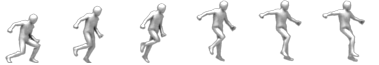
\includegraphics[width=\textwidth]{images/sprite_example/platformer_sprites_jump.png}
    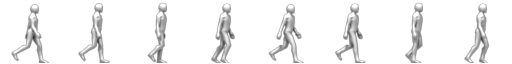
\includegraphics[width=\textwidth]{images/sprite_example/platformer_sprites_walk.png}
    \caption[Example of a 2D sprite animation]{A 2D sprite sheet used to produce a jumping animation (top row) and a walking animation (bottom row) for a human character.  The frames in this case are laid out in a single image for demonstration purposes, progressing in order starting with frame 0, the frame farthest left in this sprite sheet.  An artist may create keyframes and then fill in intermediary poses to produce a full sprite sheet as above.  These sprite sheets were created by Clint Bellanger using a 3D model and are licensed under Creative Commons Attribution 3.0, retrieved from opengameart.org.}
    \label{fig:sprite_sheet}
\end{figure}

%3D models are described as a mesh, a collection of primitive polygons (i.e. quadrilaterals or triangles) which are stored as vertices.  This mesh describes what is drawn, including any texture, color, and other material information.  Along with the mesh, a skeleton, or rig, is stored.  The rig describes a hierarchical structure of bones and accompanying joints.  Each vertex is given a series of weights describing the impact each joint has on its transformation.  This allows many vertices, and therefore many polygons, to be transformed at once in organized groups, simplifying the problem of animating the model to a matter of transforming the skeleton in the desired manner.  To animate this 3D model, an artist specifies key frames of the animation by positioning the skeleton at different time steps.  The stored key frames, instead of an image, are the transformations of each joint at this frame or step of the animation, which a rendering or game engine can interpolate between to produce the final result.

Specifying these animation frames is work intensive, taking up significant time and resources to produce for a single character.  Additionally, similar animations may need to be produced for slightly different scenarios, with only minor modifications required.  These minor modifications can be made to fit a different setting, such as a character jumping on Earth or on the moon, or can be for different characters, such as a large person moving in contrast with a small child.  Though the movement itself may be similar, manual changes must be made, requiring artist time which could be spent generating new assets.  

Recent work in animation generation seeks to automate this process, replacing the manual process with a procedural one.  Physics-based simulations can be used to produce controllers for the skeleton, determining joint positions and rotations for keyframes automatically.  Not only does this reduce the effort involved in the creation process, but this also provides a basis for dynamic interaction between a character's animation and the environment.  With manual keyframe animations this is not possible, as any specific interaction between a character and the environment must be manually created by an animator 

I present a controller that takes a skeleton as input, with additional parameters describing the character.  I then simulate a jumping motion on the character, determining a sequence of poses based on the character's muscles to produce a keyframe animation.  The additional character parameters describe the character's mass, muscles, the constraints placed on each joint to prevent unnatural rotations, and a description of the jump indicating desired time and distance.  Mass is specified per-limb, with each mass stored in the joint object affecting the limb to allow for calculation of the character's center of mass.  

\newcommand{\frameimage}[1]{\fbox{\includegraphics[scale=1.0]{#1}}}

\begin{figure}[htp]
	\centering
	\begin{subfigure}[h]{0.16\textwidth}
		\frameimage{images/jump_stages/ps1_windup.png}
		\caption{Windup}
	\end{subfigure}
	\begin{subfigure}[h]{0.32\textwidth}
		\frameimage{images/jump_stages/ps2_takeoff.png}
		\caption{Takeoff}
	\end{subfigure}
	\begin{subfigure}[h]{0.48\textwidth}
		\frameimage{images/jump_stages/ps3_airborne.png}
		\caption{In-Air}
	\end{subfigure}
	%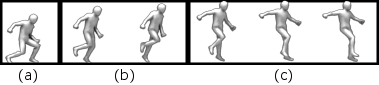
\includegraphics[width=\textwidth]{images/jump_stages/jump_stages.png}
	\caption[Example of stages of jumping]{An example 2D sprite animation of a simple human character jumping, with the jump divided into the windup, takeoff, and in-air stages.  A landing is absent from this sequence.  The windup consists of a short crouch to prepare for the jump, creating an opportunity for the body to extend and thus accelerate.  The takeoff performs this acceleration, shifting its center of mass forward past its feet and the character becomes airborne.  During the in-air phase the character moves its body to control the fall, in this case spreading its arms and shifting its feet from behind its pelvis to in front of its pelvis.}
	\label{fig:jumpStages}
\end{figure}

I divide a jump into five stages: path estimation, windup, thrust, in air maneuvering, and landing. My controller works with the initial path estimation, windup, and thrust stages of the motion as shown in Figure \ref{fig:jumpStages}.  Poses are  calculated by modeling muscles as Hookean springs attached to the skeleton at 2 points and crossing a joint as shown in Figure \ref{fig:forceCalc}. Spring constants for the muscles are specified by the user, allowing my simulation to animate characters of various strengths and body makeups.  Spring displacement from rest is calculated using the bend in the joint and constants describing the skeleton.  Using the spring displacement, a particular pose of a joint is related to the usage of the character's muscle and the elasticity of the connective tissue of the muscle and joint.

\begin{figure}[ht]
	\centering
	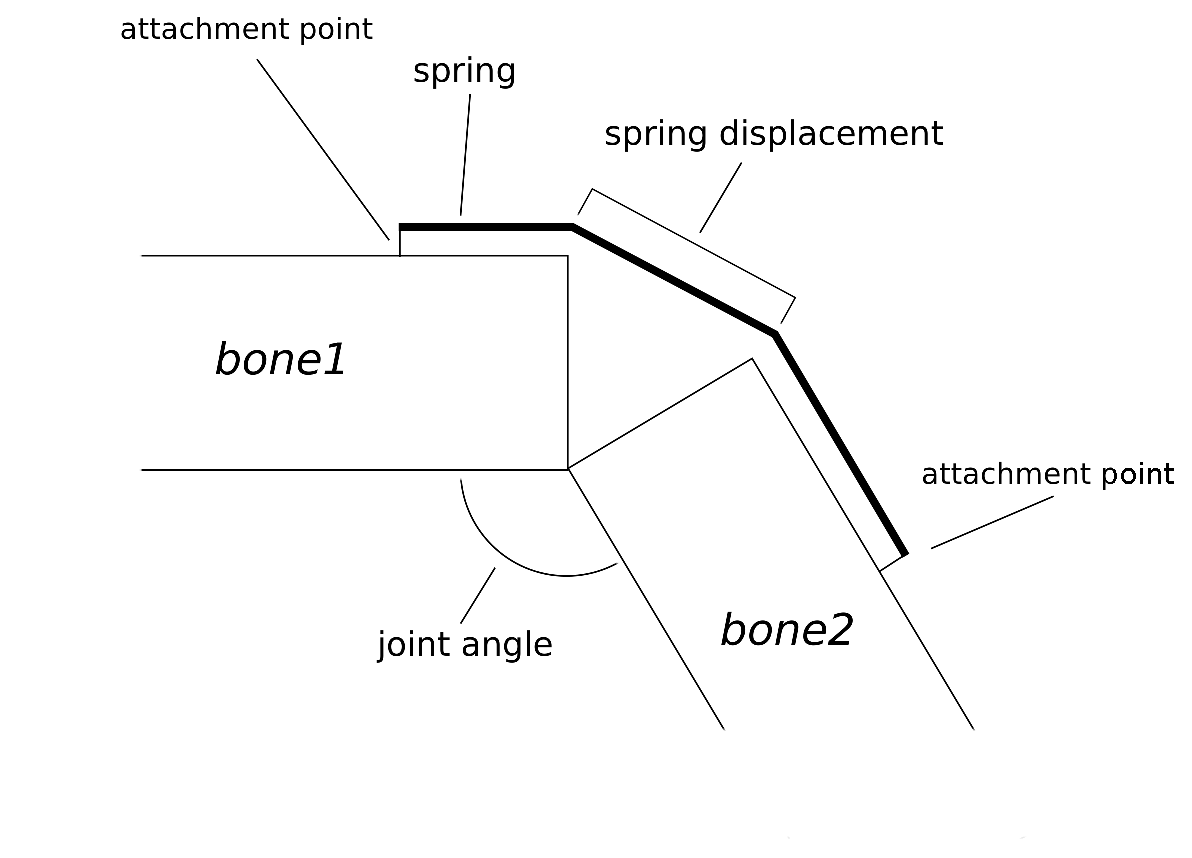
\includegraphics[width=10cm]{images/spring_calc/spring_angle_calc.eps}
	\caption[Diagram of muscle setup]{Visual representation of the setup of bones and muscles for a single joint.  This illustrates the method by which I calculate the spring displacement, taking the bones as rigid blocks which separate and stretch the string as the joint bends.}
	\label{fig:forceCalc}
\end{figure}

Two approaches are described in this thesis, one using torque and one using elastic energy.  As the springs contract, they produce forces on the bones, which result in torques at each joint.  These torques are then used to calculate a windup pose for the character by calculating resultant linear acceleration for the character's center of mass, which is compared to a calculated necessary acceleration to make the jump.  This linear acceleration is then used to compute the motion of the takeoff and in-air phases of the jump, which are sampled to create frames of an animation.  

The second approach uses the spring displacement to calculate the elastic potential energy of each muscle, which is modeled by a single linear spring.  By assuming perfect conservation of energy, I compare the total elastic potential energy of the character's muscles to a calculated necessary kinetic energy for the jump to be completed.

To control the motion and maintain plausibility, I calculate the character's center of mass and supporting polygon each frame.  This allows the character to maintain balance while flexing its joints, the position of the character's joints are adjusted to keep the center of mass positioned over the supporting polygon.  While flexing, the character constantly checks the position of its center of mass against the calculated supporting polygon, ensuring the center of mass is over the support and as close to the center as possible.

I use an inverse kinematic solver to help determine poses of intermediate joints.  This allows me to find the necessary pose for the ankle and knee of the character given the position of its foot and hip.  Many solutions in this region are possible, so I constrain the skeleton such that only those poses where the joints are within human ranges of motion are possible.

The next stage of the motion is the thrust stage where the character releases from the ground by using the potential energy of the spring-muscles to accelerate its center of mass upward.  This is handled by applying the calculated accelerations from the windup stage to the character's pelvis to accelerate the center of mass, with the inverse kinematic solver determining the poses of the legs as they unbend.  Balance must be maintained, and the relative rate of rotation of the different joints of the leg must be balanced with each other to maintain foot position while the body is transformed.  As the skeleton is a tree with its root at the character's pelvis, this can be a challenge, necessitating the use of the inverse kinematics solver.  Due to the nature of the inverse kinematics algorithm used, the extension propagates from the hip to the feet.  

The character then proceeds through the in-air portion of the jump, where the acceleration changes due to gravity before they finally land.  I assume a simple trajectory for the in-air phase, though more complex motions with turns, flips, or interaction with the environment could be created.  My simulation ends when the character's feet contact the ground, ending the in-air phase.  Other work, such as that by \liufall, has handled landing and creating a separate controller to handle this is beyond the scope of this thesis \cite{falling_landing}.

My controller is made to be a module, able to be used with other controllers as part of a larger system.  Its modularity takes the form of detecting and handling its state at each stage, consisting of its position, velocity, acceleration, pose, muscle state, and any collisions or forces applied. The controller performs actions when it has a response to its current state and ends control when it no longer has an appropriate response to allow a separate controller to handle the situation.  This allows each controller to do a smaller job well, and to act as a portion of a larger state machine handling a character's actions. Several such controllers can be connected to produce more complex animations or animation sequences, utilizing bounded starting and finishing conditions for the character as well as bounds on expected conditions during operation to allow handling of stimuli during operation.

% figure of current keyframe animation process in maya
% accompanying video for presentation
% accompanying figure/video of the resulting animation in 3d

 
\section{A Description of 3D Animation Creation}
\label{section:anim_ex}
To motivate the necessity for an automated animation method, I present an example of the method for producing an animation by hand.  First a mesh and rig must be produced, which I also require for my simulation.  This is a time and skill intensive process, requiring the artist to exercise their technical and creative knowledge and ability to create the character's figure, the mesh, and to create and attach a skeleton, the rig.  

A mesh is constructed of faces which are in turn made of vertices, and each vertex must be assigned a weight for each joint of the rig to indicate the way the vertex should transform when the joint in the rig is transformed.  These joints serve not only as a joint in the anatomical sense, but as a tracked point in the skeleton.  The joints are connected by bones, but the information is stored at the joint, which sometimes necessitates a joint to be placed in a non-anatomical way.  For example, in my rig I have a joint placed at the head, which not only allows me to rotate the head but tracks the position.  A similar situation arises with the toe and heel, where a joint is used to facilitate the placement of a connecting bone.  Once the mesh and rig are created and the weights for the rig are assigned to the mesh, an animator may create controls to manipulate several joints at once, such as creating a controller to facilitate grasping motions in which many bones of the hand must be manipulated at once.  These controls are formed from an object such as a simple spline to which several joints are constrained, allowing movement of several joints through manipulation of the control object.

Once the rig and mesh are set up, an animator must manipulate the mesh to pose the model.  Study of real subjects may be used to help ensure realism.  For a jumping motion the animator would need to decide how they want to start the animation to allow blending from other movements such as walking, running, or standing.  They must then position the model and record a keyframe.  Keyframes are hand-created frames of the animation which a renderer or game engine may interpolate between to produce a final animation, allowing an animator to create and store few frames, while still creating a smooth animation in the final setting.  This allows few frames to be stored to produce any frame rate of animation, while also reducing the storage requirements in exchange for a minor increase in computation, which is an extra interpolation for each joint in the character.

While the key frames can be sparse and there are tools for aiding in generation, this process requires heavy manual input for each animation for each character, as well as prior knowledge of the motion to be produced.  Animators commonly use live footage or subjects as a basis for their work, as done by Disney for Snow White, which used footage of Marge Champion, and animal references for the Lion King \cite{disney_art, disney_hist}.  Life drawing is also used as a practice or reference for hand drawn animation \cite{camara_anim_tech}. Characters that move differently due to differences in weight or body makeup must be animated separately, requiring an artist to perform similar, time consuming work.  For example, a character with extremely strong legs may bend less, applying the same force as a weaker character over a shorter distance to achieve the same acceleration.  A heavier character would need to apply much more force to achieve the same acceleration and thus jump height as a lighter character, necessitating stronger muscles or a greater distance over which the force is applied, thus requiring a deeper squat than the light character.  With a simulation-based approach this work could be reduced, especially repeated work, to setting variables such as weight, height, and musculature for the different characters and generating the set of animations desired.  As techniques and technologies improve, a simulation could be used in place of a stored key frame animation, creating the animation in place based on its environment and situation, thus shifting the burden on an animator from preparing poses and keyframes to adjusting body dimensions, weight, strength, and constraints.

For a jump specifically, a human loads the muscles in their legs, quickly moving to a particular bend based on the feedback they feel in their muscles and joints, as well as balance feedback and their knowledge of the jumps they have performed in the past.  The appearance of bearing and lifting weight is difficult to achieve, as the animator must visually match the poses to their knowledge of bodies or to a visual of a similar human to their character performing the motion.  Simulation allows a computer to calculate movement based on physical aspects of the character, incorporating knowledge such as the character's weight and body make up, allowing an animator to produce animations of unfamiliar motions with a higher degree of physical plausibility.

% explain contributions
% - what is the contribution of this technique
% - Unity3D -> what am I getting from outside sources
% - what am I making myself

\section{Contributions}
\label{section:contributions}
	This thesis describes a controller which simulates a jumping motion of a character.  The generated animation is created to be plausible in appearance, using a simplified physical representation.  I sacrifice some physical accuracy in favor of speed and simplicity of creating, describing, and implementing the simulation.  Specifically, I contribute a description for the windup, thrust, and in air phases of a jump and created a controller using a physical simulation and an implementation in \unity{}.  In short, my contributions are:
	\begin{itemize}
		\item A controller which simulates a windup and thrust phase of a jump, moving the character from the ground into the air
		\item A description of character poses based on torque generated by muscles
		\item A description of character poses based on elastic energy of the muscles
		\item A sampling-based method for choosing a pose given muscles and a desired output
		%\item Estimates and quantification of ``good'' values for spring constants
		\item Visualizations of the animations and values for analysis and presentation
	\end{itemize}

\section{Summary}
\label{section:intro_summary}
In this chapter, I introduced the problem of animating a character to perform a jump motion and the simulation-based approach to animation.  I then presented an example of a current method of creating animations in Section \ref{section:anim_ex}, describing how an artist would create a character and animate it for a video game or film.  I then gave a summary of the contributions of this thesis.

Expanding on the ideas introduced in this chapter, Chapter \ref{chapter:previous_work} discusses existing work in simulation, motion capture, and inverse kinematics which inspired and directed the work of this thesis.  Chapter \ref{chapter:animation} discusses my method, describing the torque-based and energy-based simulations I used to produce animations.  Visualization for debugging, understanding, and presenting these animations is discussed in Chapter \ref{chapter:visualization}, and the results themselves are discussed in Chapter \ref{chapter:results}. Lastly, I discuss future work and draw final conclusions in Chapter \ref{chapter:future_work}. 	% chapter 1

%%%%%%%%%%%%%%%%%%%%%%%%%%%%%%%%%%%%%%%%%%%%%%%%%%%%%%%%%%%%%%%%%%% 
%                                                                 %
%                           PREVIOUS WORK                         %
%                                                                 %
%%%%%%%%%%%%%%%%%%%%%%%%%%%%%%%%%%%%%%%%%%%%%%%%%%%%%%%%%%%%%%%%%%% 
 
% \specialhead{PREVIOUS WORK}
\chapter{PREVIOUS WORK}
\label{chapter:previous_work}
In this chapter, I introduce previous work in the field that inspired and directed my work. First I discuss the production of animation using motion capture in Section \ref{subsection:mocap_bg}, then muscle-based simulations in Section \ref{subsection:muscle_sim_bg}.  Muscle-based simulations were a major inspiration for my work, as well as rigid-body simulations that control the character through means other than muscle simulations which I describe in Section \ref{subsection:rigid_body_bg}.

\section{Background of Computer Generated Animation}
\label{section:computer_gen_bg}
\subsection{Motion Capture}
\label{subsection:mocap_bg}
Producing athletic animations for human characters is difficult.  Motion capture is one method used for production of realistic animations for human athletics and other motions. Cameras are used to capture the movements of live actors that are then applied to 3D models, allowing the actor's performance to control the virtual character.  In marker-based capture, numerous tracking points are attached to the actor, aiding a system of connected cameras in following the movements of the actor.  Other methods attempt pose estimation without markers by extracting silhouettes and edges of the actor from images, though these methods are less capable of capturing detail. Richard Radke gives an overview of these methods, as well as of the necessary calibration of the systems and processing of the data collected \cite{radke}.

In marker-based capture optical marks are worn by the actor.  These marks are then used to determine the position of the actor in 3-dimensional space by a set of cameras surrounding the actor.  The camera system must be calibrated before capture can be performed.  The markers are then tracked by the camera system, estimating positions in space by leveraging multiple cameras' views of a each marker.  One method of tracking these markers is framed as a learning problem as per Liu and McMillan, using principal component analysis to build a linear model \cite{liu_mocap}.  

After acquiring the marker data, the pose of the body is estimated using forward kinematics.  Inverse kinematics is then used to determine the angles of the skeleton's joints from the tracked positions of the skeleton.  I use inverse kinematics as part of my simulation, and so discuss relevant background in Section \ref{subsection:ik_bg}.  However, the problem for motion capture is slightly different as the skeleton is usually over-constrained by many markers, as opposed to the inverse kinematics problem in my simulation where the problem is to position a handful of points on the skeleton at specified target positions.  The same principles apply in these situations, but utilize cost functions to minimize error across the entire set of markers and learning models to determine the most likely motion the actor is performing.

The motion captured must then be applied to the virtual model.  Several separately recorded motions may need to be blended together to produce longer animation sequences, requiring interpolation and blending between captured motions.  Witkin and Popovi\'{c} provide one method for blending and editing both keyframe and captured animations using motion curves, which are descriptions of the parameters of the model over time.

In marker-less capture, the images are segmented to determine the position of the actor.  Depth sensing may be used, such as that described by Shotton et al \cite{shotton_kinect}, which is used in the Kinect created by Microsoft.  This method utilizes a large amount of training data, both captured from humans and synthesized, to build a decision forest to be used for classification.

Motion capture overall provides a strong method of creating realistic animations for characters, but has several shortcomings.  For each animation desired, a capture must be made, requiring large amount of actor or performer time.  Additionally, the equipment for motion capture systems can be costly both in money and time, requiring large amounts of setup and calibration for a capture session.  These motions also require positioning of markers for detailed capture, necessitating props and prostheses in cases where the actor is not proportioned like the character desired, e.g. when an actor plays another species with longer limbs than a human.

\subsection{Muscle-based Simulation}
\label{subsection:muscle_sim_bg}
Another method of producing animations simulates a complex muscle model mimicking the biology of the human body. Muscle-based approaches produce realistic motions which adapt to the environment, using a complex model of the musculo-skeletal structure. These methods are often complicated to produce, requiring learning methods and complex constructions of the character's body, though they react well to applied stimuli and are often flexible in the animations produced.

Grzeszczuk and Terzopoulos produce animations of animals, mostly those with many degrees of freedom such as fish, by producing actuator control functions for the muscles of the controlled character \cite{fish_muscles}.  An objective function provides feedback which can then be used to learn muscle activations, modeling neural signals, required to produce motions.  Controllers are then learned for low-level tasks such as moving at different speeds and turning.  By composing numerous learned controllers, complex motions are produced such as a fish jumping out of the water.

Geijtenbeek et al.\cite{muscle_based_bipeds} use a rough, user-created muscle routing on a skeleton to produce various gaits that are learned based on the velocity and environment.  The muscle routing is optimized to remain within a physical region while providing optimal forces on the skeleton based on freedom of motion of the skeletal joints and the calculated optimal length of the muscle.  This model is then used to compute sequences of muscle activations that produce the final animations.  This method is effective, producing good results in various levels of gravity on at least 10 different bipedal skeletons which can react to external stimuli.

My simulation utilizes a muscle-based approach, though in a simpler manner than in the work described above.  I use a simplified muscle model to reduce user-specified biology and to reduce complexity of the problem of moving the character. By avoiding a learning method, I reduced time spent on precomputation and also attempted to reduce overall compute time to achieve interactive performance.  I chose the simpler model also to limit the scope of this thesis, though attempting similar work with a learning model and complex muscle model would provide interesting work in the future.

%\begin{figure}[htp]
	%\centering
	%\includegraphics[width=0.2\columnwidth]{muscle_based/muscle_routing.eps}
	%\caption{Example of a muscle routing on a skeleton from Geijtenbeek et al. \cite{muscle_based_bipeds}.}
%\end{figure}
		
%\begin{figure}[htp]
	%\centering
	%\includegraphics[width=0.3\columnwidth]{falling_motion/falling1.eps}
	%\hspace{0.1\columnwidth}
	%\includegraphics[width=0.3\columnwidth]{falling_motion/falling3.eps}
	%\caption{Breakdown of a hands-first falling approach from Ha et al. \cite{falling_landing} and of a feet-first landing approach.  Ha et al. use a rolling strategy to minimize stress on the body and produce a realistic fall.}
%\end{figure}


\subsection{Non-Muscle Simulations}
\label{subsection:rigid_body_bg}
Instead of complex muscle systems, some physical simulations utilize a rigid-body character with a user-defined skeleton to find optimal poses based on desired conditions other than muscle simulation.  \liufall{} utilize such a scheme to generate landing motions for human characters based off linear velocity, global angular velocity, and angle of attack  \cite{falling_landing}.  The system chooses either a feet first or hands first landing strategy and moves into a roll to reduce stress on the body using principles from biomechanics and robotics.  A sampling method is applied to determine successful conditions, producing bounding planes for the data.  The movement is broken into stages of airborne and landing, in which the character re-positions for the designated landing strategy, and executes the landing strategy respectively. Each of these is separated into impact, roll, and get-up stages.  Movement and joint positions are produced using PID servos.  

Other work on producing such controllers was produced by Faloutsos et al. who described a method of composing such controllers by giving pre-conditions, post-conditions, and intermediate state requirements \cite{composable_controllers}.  The composed controllers are then chosen at each step based on the current pose and which controller is deemed most suitable.  By providing a state-machine-style construction for the controllers, they create a way to build many smaller controllers into a more complex motion.

Hodgins et al. created several controllers for running, vaulting, and bicycling, creating realistic motions and secondary motion using rigid bodies and spring-mass simulations \cite{anim_human_athletics}.  Geijtenbeek and Pronost provide a detailed review of physics based simulations \cite{inter_physics_anim}.

Koga et. al use path planning, inverse kinematics, and forward simulation to generate animations of arm motions for robots and humans working cooperatively.  They produce arm manipulations that avoid collisions and result in final positions and orientations for specified parts of the arm to produce motions such as a human putting on glasses and a robot arm and human cooperating to flip a chessboard \cite{motion_intentions}.

My work was inspired heavily by these simulations, though I chose to incorporate muscles into the simulation.  These control schemes helped inspire the method of control and optimization used in my simulation.  The descriptions of controllers as modules that can be fit together into a larger state machine of controllers to handle many situations led to the creation of my controller as one such module, intended to be used alongside other controllers for handling landing and in-air maneuvers such as that created by \liufall{}.

\subsection{Inverse Kinematics}
\label{subsection:ik_bg}
Solving the inverse kinematics problem is necessary to my simulation for positioning of the feet.  As described in Section \ref{section:ik} in more detail, the setup of my skeleton requires a method of posing the character such that if the pelvis is moved to a different position, the character's feet remain in the same place.  Several different methods exist of varying complexity.  A simple, cyclic-coordinate-descent method allows solving for a single chain of joints as described by Lander \cite{kine1, kine2}. A detailed description of this method can be found in \ref{section:ik}.  This method was chosen for simplicity and the minimal extra infrastructure required, as other methods required matrix math libraries not easily available.

Buss surveys inverse kinematics methods, describing the classical Jacobian transpose, Jacobian pseudoinverse, and damped least squares methods \cite{buss_ik}.  End effectors are defined as particular points on the skeleton.  The positions of the end effectors are defined by the joint angles of the skeleton.  The Jacobian matrix is a function of the angles of the joints, describing the relationship between the joint angles and the position of each end effector.  The Jacobian for a particular state of the skeleton can be computed, with further Jacobian matrices computed by choosing changes in the angles of the skeleton.  The inverse of the Jacobian gives a value for this choice of change.  As the Jacobian is likely not invertible, approximations and alternatives are used.  The transpose provides a fast approximation, though it is a different solution than the inverse.  The pseudoinverse provides a good, fast approximation, but lacks stability around singularities.  The damped least squares method avoids this issue of stability by incorporating a damping constant.

Another method by Aristidou and Lasenby frames the problem as finding a point on a line \cite{fabrik}.  The system, termed Forward And Backward Reaching Inverse Kinematics (FABRIK) uses an iterative approach.  Iterating over the the joints of the body, the algorithm repeatedly finds a new joint position along the line between the current and desired positions with an appropriate distance from its neighbor.  Which neighbor is used for calculation is determined by if the iteration is currently working forwards or backwards.

\section{Commercial Software}
\label{section:commercial_bg}
Several technologies exist to similarly aid in animation production. \unity{} Mecanim applies constructed animations of various types to similar skeletons, providing joint constraints and muscle definitions in a similar manner to my simulation \cite{unity_mecanim}.  MecAnim provides functionality for constraining range of motion and blending between existing animations, utilizing existing clips to produce complex animations in a manner similar to the composable controllers described by Faloutsos et al., as well as inverse kinematics solving.  Due to a lack of understanding of the features and limitations, as well as what level of control is available, I chose not to utilize Mecanim for my current implementation.  As discussed in chapter \ref{chapter:future_work}, future work would ideally take advantage of Mecanim.

3ds Max footsteps offer a method of positioning feet and producing walk, run, and jump cycles based on  number of parameters \cite{3dsmax}.  Without knowledge of the algorithm, analysis is difficult, but it seems to produce animations by specifying timing and parameters about the stride.  Parameters defined include stride width, length, and height.  My simulation seeks to produce more natural looking animations through use of a muscle simulation.  The footstep style of animation may be preferable to artists however as it gives very strong control over the timing and spacing of the individual events of the animation, such as foot falls.

\section{Summary}
\label{section:background_summary}
In this chapter I discussed the previous works that guided my research as well as existing solutions to the problem of animating characters. I discussed existing work in motion capture, which offers a method of producing realistic animations, but must be performed offline and requires significant actor time as well as setup of a capture system.  I described muscle and non-muscle simulations used to generate animations, both of which inspired the work described in Chapter \ref{chapter:animation}, and discussed approximate solutions to the inverse kinematics problem, which is expanded upon in Section \ref{section:ik}.  Finally, I discussed some existing solutions and tools in commercial software which perform similar tasks to the work in this thesis, but ultimately fill different roles in the production of animation.  In the next chapter, I discuss my simulation in detail.

%%%%%%%%%%%%%%%%%%%%%%%%%%%%%%%%%%%%%%%%%%%%%%%%%%%%%%%%%%%%%%%%%%% 
%                                                                 %
%                           METHODS                               %
%                                                                 %
%%%%%%%%%%%%%%%%%%%%%%%%%%%%%%%%%%%%%%%%%%%%%%%%%%%%%%%%%%%%%%%%%%% 
 
% \specialhead{METHODS}
\chapter{VISUALIZATION}
\label{chapter:visualization}

% talk about instpiriations here instead of prev work

\section{Motion Visualization}
\label{section:motion_vis}
For visualizing motion of a character or figure, there are a limited selection of different techniques.  Most common is a sequence of frames in which a character is posed, either in a still sequence or as a video.  As this is a final goal of our system, this is a valid visualization, but fails to provide a simple comparison between one animated sequence and another.  This is desirable for qualifying or quantifying performance of the system.  A sequence of still images is also space-consuming, which can be undesirable for print formats or even digital formats where length or size of document is an issue.

Specific markers can be used to highlight motion of particular parts of the body, such as the pelvis or center of mass.  Other indicators placed on or around the figure can indicate other values, such as arrows to represent vectors of force.  This however can result in clutter within the images, scene, or frame of video, occluding or distraction from the primary animation.
%TODO motion sculptures, see vimeo likes
% the motion sculptures are previous work, but the rest is something I just kind of tried, is that a previous work? should this whole section just be under visualization?

\section{Summary}
\label{section:vis_summary}

\chapter{MAGNIFICATION}
\label{chapter:magnification}
This chapter details the main contribution of this thesis work: the magnification effect generated by manipulating the distances for both the texture and the graph network. Subsection~\ref{section:texture_magnification} explains the process used in transforming the rendered FBO texture that the satellite images (Section~\ref{section:satellite_images}) and road network (Section~\ref{section:road_network}) both render to.

The requirements for this non-linear magnification of a texture include the ability to specify an inner and 
outer radius of magnification as well as a linear zoom factor. The program is intended to create a visual
effect such that the non-linear region between the inner and outer radii smoothly blends the regions of linear
zoom and base level magnification. The resulting function that accomplishes these goals should be easily
extensible to allow for multiple cursors interacting with the system at the same time. 

In performing magnification, we attempt to show more information to the users while ensuring that the data is still continuous. Some data loss will occur as regions become demagnified, but we attempt to minimize this as much as possible. As noted by Keahey and Robertson, our piecewise function should be continuous on its boundaries: the linear and non-linear functions should return the same value at the inner radius, and the non-linear function should return the input
value at the outer radius \cite{Keahey1996}.

A similar transformation is applied to the nodes and endpoints of line segments for the graph network. As mentioned previously in Chapter~\ref{chapter:intro}, most of the data in the graph network corresponds to
physical locations, so when the underlying satellite images get transformed by the texture magnification, the 
nodes and line segments must move accordingly. This process is explained in 
Subsection~\ref{section:graph_magnification}.

\section{Texture Magnification}
\label{section:texture_magnification}

To simulate magnification when dealing with rendering textures, we perform transformations the entire FBO texture
based on proximity to mouse cursors. Given three values, an inner radius, \emph{$r_0$}, an outer radius, 
\emph{$r_1$}, \emph{z}, a linear zoom factor, we construct two different formula for performing either a linear 
or non-linear magnification.

\begin{figure}[htp] \centering
    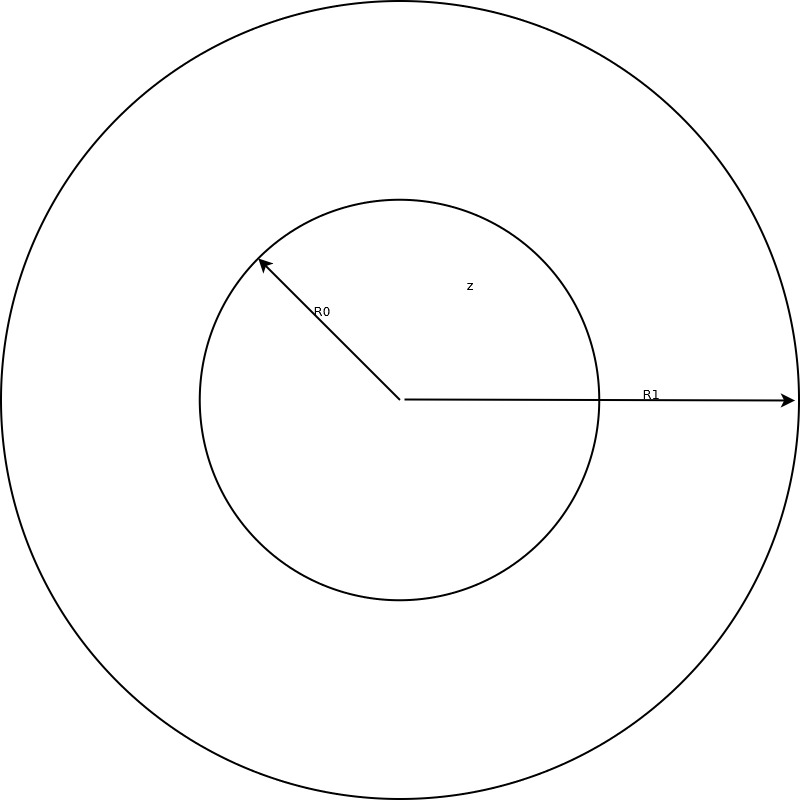
\includegraphics[width=0.4\linewidth]{img/cursor_mag.jpg}
    \caption[Magnification Parameters]{Visualization of the magnification parameters. \emph{z} is the linear zoom factor, \emph{$r_1$} is the outer radius, and \emph{$r_0$} is the inner radius.}
    \label{fig:mag_parameters}
\end{figure}

In both types of magnification, given the distance, \emph{d}, from a particular mouse cursor, $\vec{c}$,  to the 
original UV coordinate for a particular fragment, $\vec{p}$, the equations return a new scaled distance. This new 
distance, $f(d)$ is multiplied by the normalized direction vector between the mouse cursor, seen in
Equation~\ref{eq:magnifying_vector}.

\begin{equation}
    \label{eq:magnifying_vector} 
    v_i = f(d) \times \frac{\vec{c_i} - \vec{p}}{|\vec{c_i} - \vec{p}|}
\end{equation}

For distances less than \emph{$r_0$}, we perform linear magnification. The equation for which is given in 
Equation~\ref{eq:linear_magnification}

\begin{equation}
    \label{eq:linear_magnification}
    f(d) = d \times \frac{1}{z}
\end{equation}

We scale the distance by $\frac{1}{z}$ due to how UV sampling is performed. Reducing the area of the sampled 
texture spreads less information over the same area, resulting in the ability to see more data. An example of this is shown in Figure~\ref{fig:UV_sampling}.

\begin{figure}[htp] \centering
    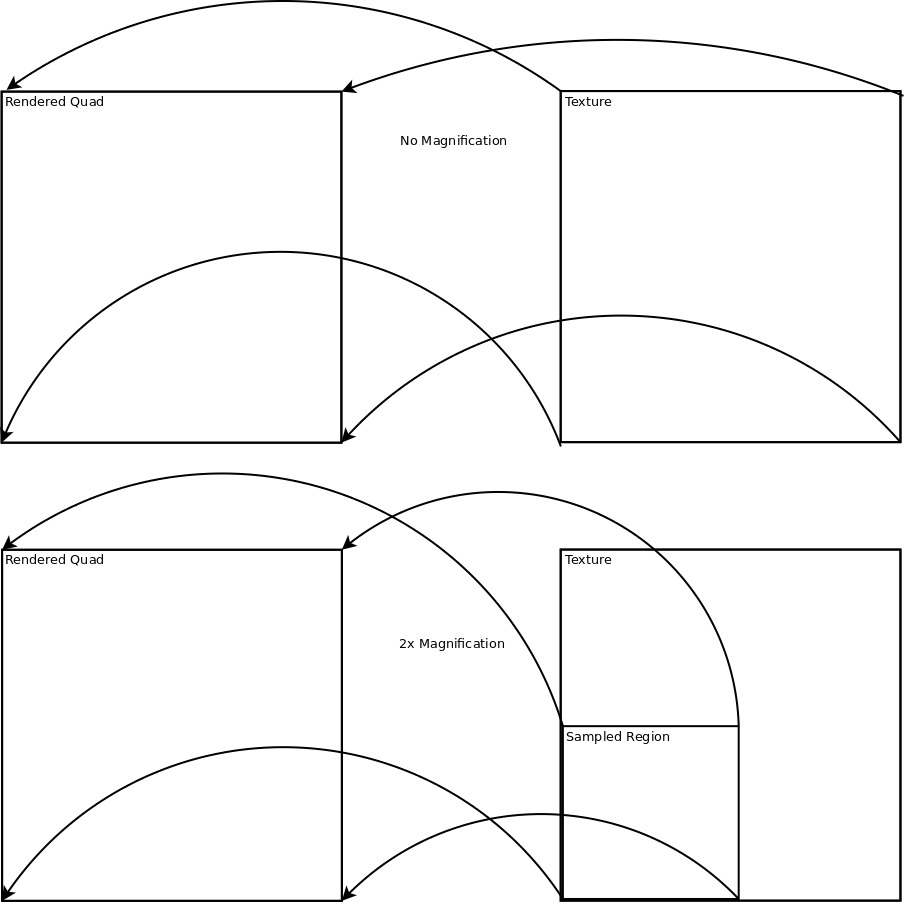
\includegraphics[width=0.6\linewidth]{img/texture_mag.jpg}
    \caption[UV Sampling]{Simple UV sampling example demonstrating magnification. The texture remains the same, we simply sample from a smaller region when performing magnification.}
    \label{fig:UV_sampling}
\end{figure}

For distances less than \emph{$r_1$}, we use the same premise of Equation~\ref{eq:linear_magnification}, but 
scale the linear zoom factor based on the distance away from the center instead of using a fixed value. To 
achieve this goal of a smooth, continuous image, we need a function which is continuous and has a smooth derivative. There are a few functions which follow the general form of having upper and lower limits; functions with a sigmoidal shape fall into this category. For our purposes, the desirable features are a smooth but rapid decrease from the higher magnification level, \emph{z} to the baseline level, 1. 
The generalized logistic function (Equation~\ref{eq:logistic_function}) fits these requirements as seen in 
Figure~\ref{fig:logistic_graph}, and is modified to fit our parameters, shown in 
Equation~\ref{eq:modified_logistic}

\begin{equation}
    \label{eq:logistic_function}
    f(x) = \frac{1}{1 + ae^{-bx}}
\end{equation}

\begin{equation}
    \label{eq:modified_logistic}
    f(d) = d \times \left( 1 + \epsilon + \frac{(z - 1 + 2\epsilon)}{1 + ae^{b(d-r_0)}}\right)
\end{equation}

The variables, \emph{a} and \emph{b}, can be solved for with the following two equations,~\ref{eq:solve_a} and~\ref{eq:solve_b}, essentially using a known given point to solve for the two variables.

\begin{equation}
    \label{eq:solve_a}
    a = \frac{\epsilon}{z - 1 + \epsilon}
\end{equation}

\begin{equation}
    \label{eq:solve_b}
    b = \frac{ln\left( \frac{\frac{z - 1 + 2 \epsilon }{\epsilon} + 1}{a}\right) }{r_1 - r_0}
\end{equation}

\begin{figure}[htp] \centering
    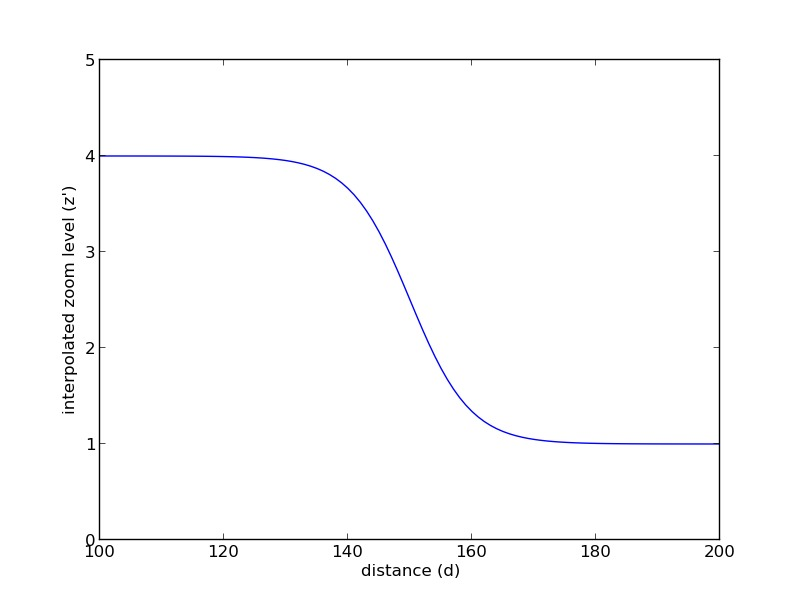
\includegraphics[width=0.8\linewidth]{img/logistic_graph.jpg}
    \caption[Logistic Graph]{Example graph of a logistic function with $\emph{$r_0$} = 100$, $\emph{$r_1$} = 200$, and $\emph{z} = 4$.}
    \label{fig:logistic_graph}
\end{figure}

The combined piecewise function for the distance function is shown below (Equation~\ref{eq:piecewise}).

\begin{equation}
    \label{eq:piecewise}
    f(d) = \left\{
        \begin{array}{lcr}
            d \times \frac{1}{z} & : & 0 < d < r_0 \\
            d \times \left( 1 + \epsilon + \frac{(z - 1 + 2\epsilon)}{1 + ae^{b(d-r_0)}}\right) & : & r_0 < d < r_1\\
            d & : & r_1 < d 
        \end{array}
    \right.
\end{equation}

A graph of the distances for the texture magnification functions is shown below in 
Figure~\ref{fig:texture_mag_graph} comparing the original distance and the computed distance.

\begin{figure}[htp] \centering
    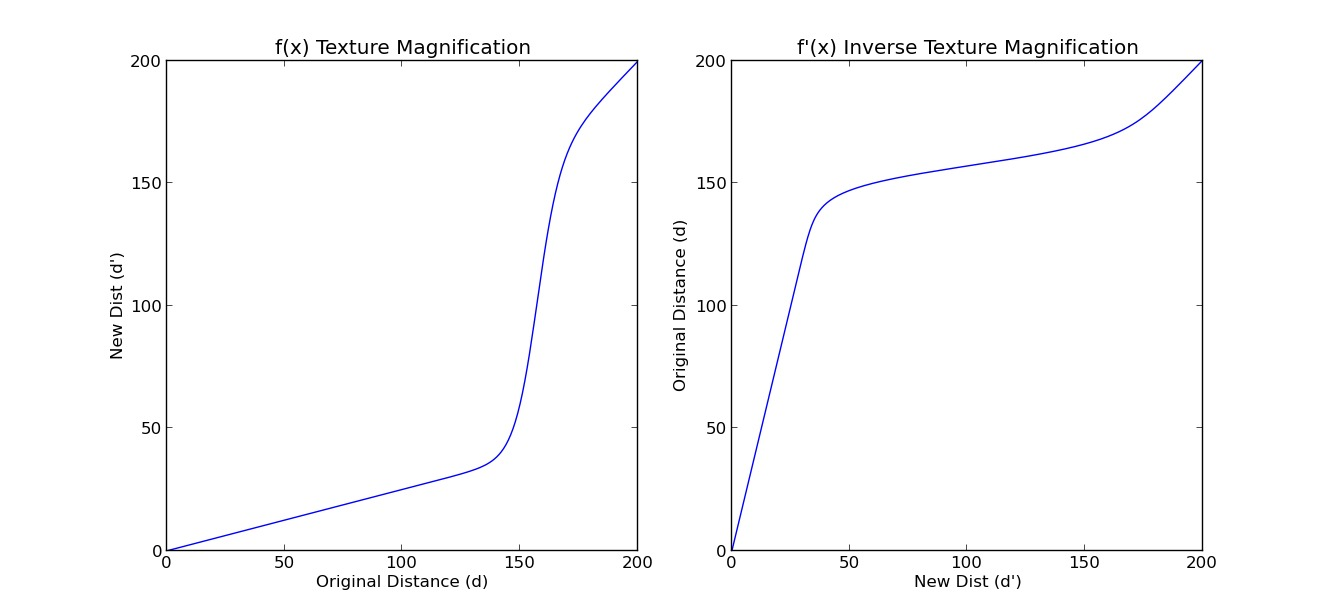
\includegraphics[width=0.8\linewidth]{img/full_graph.jpg}
    \caption[Distance Function]{Graph of the piecewise function, the x axis represents the original distance from 
    the mouse cursor and the y axis represents the new computed distance from the mouse cursor. The right image 
    is the graph of the inverse of the piecewise function. This figure shows that both functions have the same 
    domain and range.}
    \label{fig:texture_mag_graph}
\end{figure}

\section{Graph Magnification}
\label{section:graph_magnification}
To move the graph network correctly, we must use functions that are related to the texture magnification 
functions above. To perform magnification on a texture, we decrease the distance between the original UV coordinate and the focal point. If we decrease the distance between a cursor and a graph element, we cause the data to become clustered around the cursor instead of moving further away from the cursor.

Both functions map to the same domain and range. For any input between 0 and the outer radius, $r_1$, the output 
of the distance function should also be between 0 and $r_1$. The function for moving the graph network is also 
piecewise, much like the texture magnification functions.

If we examine the linear magnification function and its inverse for texture magnification, we can deduce that the correct way magnify the graph network is the 
inverse of the texture magnification function. The inverse of the linear magnification transformation (seen in 
Equation~\ref{eq:linear_magnification}) is trivial to compute, and is shown below in 
Equation~\ref{eq:inverse_linear_magnification}. The original function transforms values in the range of 0 to 
$r_0$ to 0 to $\frac{r_0}{z}$, so the inverse equation only accepts inputs in the range 0 to $\frac{r_0}{z}$.

\begin{equation}
    \label{eq:inverse_linear_magnification}
    g(d) = d \times {z}
\end{equation}

While the linear equation is trivial to invert, the logarithmic function is impractical to do analytically. The 
simplified version of the non-linear texture magnification is shown in Equation~\ref{eq:simple_log}. Solving this 
problem requires using Lambert W functions \cite{Corless1996}. Solving this equation was outside of the scope of the thesis, so we avoid solving this problem analytically by solving Equation~\ref{eq:modified_logistic} and storing the values in an 
array. Retrieving the values from the array uses a binary search to find the solution. For our purposes, we stored every value in the range from $r_0$ to $r_1$ with an interval of $0.1$. This interval was discovered by viewing the derivative of the texture magnification function.

\begin{equation}
    \label{eq:simple_log}
    f(d) = de^{d}
\end{equation}

The full piecewise function for graph magnification is seen below, $BinarySearch(z,d)$ corresponds to the index in the table given by performing a binary search of the table with a zoom level, \emph{z}, for a particular distance, \emph{d}. Because we only store values from $r_0$ to $r_1$, we add $r_0$ to this value to get the answer for the inverse of the non-linear function.

\begin{equation}
    \label{eq:inv_piecewise}
    g(d) = \left\{
        \begin{array}{lcr}
            d \times z & : & 0 < d < \frac{r_0}{z} \\
            BinarySearch(z,d) + r_0 & : & \frac{r_0}{z} < d < r_1\\
            d & : & r_1 < d 
        \end{array}
    \right.
\end{equation}


\section{Multi-cursor Magnification}
\label{section:multi_cursor}

The techniques described in the previous sections (Section~\ref{section:texture_magnification} and~\ref{section:graph_magnification}) are all applicable for
situations where only a single mouse cursor is applied within $r_1$ pixels of the cursor. The formulas 
described above are extensible and only need to be modified slightly for usage when multiple cursors affect
a fragment or graph element.

Intuitively, we would expect that cursors closer to a point should have more of an effect on the final
position of a fragment or graph element than cursors that are further away. This intuition leads to one possible
solution of performing a weighted average to get a final position.

Instead of simply returning a new distance from the texture and graph magnification functions 
(Equations~\ref{eq:piecewise} and~\ref{eq:inv_piecewise}), we have each function return two values, 
the original distance and the vector corresponding to the direction it would have been moved in. 

Because we want cursors that are closer to the element being affected to have a stronger influence, we
assign a higher weight to cursors that are closer, a full equation is seen below 
(Equation~\ref{eq:weighted_cursors}). It is important to note that the weights add up to 1.0, as we should not
move a point more than it can be transformed by the single application of the magnification equations.

\begin{figure}[htp] \centering
    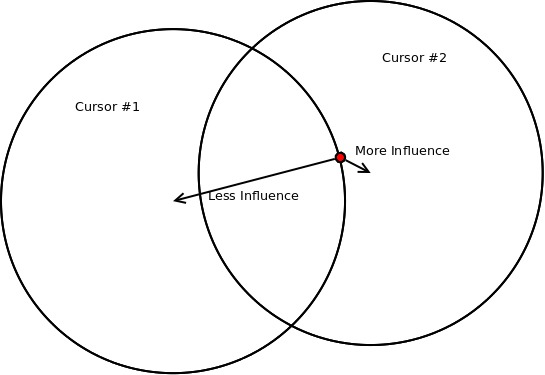
\includegraphics[width=0.6\linewidth]{img/multi_cursor.jpg}
    \caption[Multiple Cursor Magnification]{The two regions of magnification are seen overlapping a particular red point. Cursor 2 should have a higher weight when determining the final position, as it is closer to the original position of the point.}
    \label{fig:multi_cursor}
\end{figure}

\begin{equation}
    \label{eq:weighted_cursors}
    w_i = \frac{r_1 - d_i}{\sum\limits_{i=1}^n (r_1 - d_i)}
\end{equation}

\begin{equation}
    \label{eq:weighted_sum}
    \vec{v'} = \sum\limits_{i=1}^n w_i \vec{v_i}
\end{equation}

The vectors are multiplied by the corresponding weight, and the resulting vector is added to the original point
to get the new position of the element (Equation~\ref{eq:weighted_sum}). $\vec{v_i}$ the result of multiplying
the result of the piecewise function (Equation~\ref{eq:piecewise}) for texture magnification or graph manipulation
(Equation~\ref{eq:inv_piecewise}) by the normalized direction to the cursor $\vec{c_i}$.

\begin{figure}[htp] \centering
    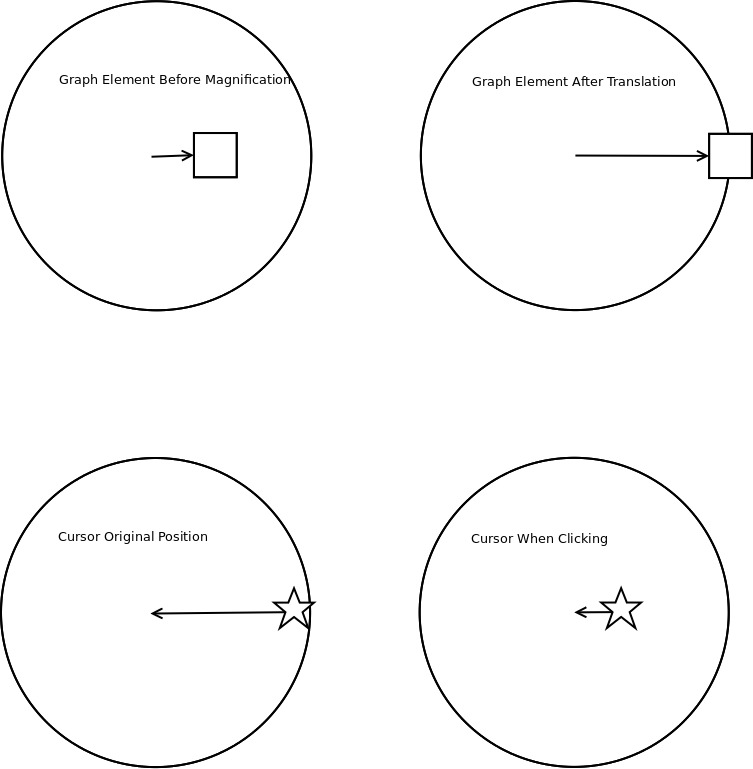
\includegraphics[width=0.6\linewidth]{img/clicking.jpg}
    \caption[Interacting with Magnified Elements]{The circular region represents the area magnified by a cursor at its center. The magnification that moves the graph element must be inverted to allow users to click on the actual position of the graph element, as seen in the bottom half of the image.}
    \label{fig:clicking}
\end{figure}

When interacting with the visualization application without magnification, every cursor is assumed to be directly over a point in screen space. However, when graph elements are moved due to being magnified by a cursor, we must compensate for the magnified position to interact with the node accordingly. Seen in Figure~\ref{fig:clicking}, we perform the texture magnification equations on a cursor to find the original position of a graph element. This occurs only when clicking on a graph
element, the cursor does not actually change its position on the screen.

\section{Summary}
\label{subsection:magnification_summary}

This chapter detailed the main magnification function used for our application for both satellite images and the graph network. A method for applying this function when multiple points of focus are included is also described. The following chapter discusses the application's overall performance and a short survey of responses to the new system.


%%%%%%%%%%%%%%%%%%%%%%%%%%%%%%%%%%%%%%%%%%%%%%%%%%%%%%%%%%%%%%%%%%% 
%                                                                 %
%                           RESULTS                               %
%                                                                 %
%%%%%%%%%%%%%%%%%%%%%%%%%%%%%%%%%%%%%%%%%%%%%%%%%%%%%%%%%%%%%%%%%%% 
 
% \specialhead{INTRODUCTION}
\chapter{RESULTS}
\label{chapter:results}
In this chapter we discuss results of our simulation.  First in Section \ref{section:pd_constants_results}, we describe choosing of the constants for the proportional derivative controllers, which required proportional ($k_p$) and derivative ($k_d$) constants to control the rate at which changes were applied to the simulation, motivating the choice of values in Table \ref{tab:pd_constants}.  We then discuss choice of muscle strength constants, as well as the length and height of trial jumps in Section \ref{section:muscle_results}.  This section also gives an estimate for how strong a human leg with similar dimensions would be.  Section \ref{section:speed_frame_results} describes performance of the simulation as well as our method of collecting frame data.  Examples of this collected frame data is shown in Section \ref{section:image_results}.  Finally, we discuss limitations of our simulation and method in Section \ref{section:limitations}.

\section{Proportional Derivative Controller Constants}
\label{section:pd_constants_results}
The windup PD controller was given constants of $k_p = 0.25$ and $k_d = 0.25$.  These were chosen empirically to offset irregularities due to time step and slow convergence in the inverse kinematic solver.  With higher values, the translation of the pelvis results in the character's feet embedding in the ground plane due to too great a movement in a single frame.  The feet then fail to adjust as the inverse kinematic solver cannot converge quickly enough.  As opposed to a performance issue, this is a limitation of the inverse kinematics algorithm used, which was chosen due to simplicity so focus of this project could remain on the jump simulation.  

In most cases, the inverse kinematic solver converged within 30 iterations, but in this situation more than 300 iterations were required.  To compensate, we chose PD controller constants to adjust the rate of of change of the animation.  These values were found to generally produce smooth windup phases without compromising on speed of the animation too much, where speed refers to the amount of movement in each frame, which requires the frames to be played back at a different rate to achieve the desired rate of movement in the final animation.

The controller for re-balancing performed well with $k_p = k_d = 1$, with little noticeable change in results and only a change in rate of convergence for values at $k_p = k_d = 0.5$ and $k_p = k_d = 1.5$.  This showed that the main bottleneck for control in the model was the windup control, leading us to choose the value 1.

\section{Muscle Constants and Strength Intuition}
\label{section:muscle_results}
Muscle spring constants were tested in various configurations, with several trials run for each set of constants for varying distances, directions, and situations.  Animations were created for forward jumps between 1m and 2m for the normal human values and at 1m, 10m, and 100m for the super human, based on the analysis of the standing long jump by Wu et al\cite{longjump}.  A jump onto a box was also simulated, with 0.5m and 0.75m boxes for the normal human and 1m and 100m boxes for the super human, with normal human values chosen based on the work done by Arag\'{o}n-Vargas and Gross \cite{vertjump}.  The normal human muscle constants were additionally used for sideways jumping animations, as well as a more complex scene in which the character is made to jump from on top of a box, over an obstacle before finally landing on the ground.

%biomechanics of sport and exercise
Jump animations appear plausible, and the spring values result in forces similar to a human muscle.  Human muscles have about $30\frac{N}{cm^2}$ force per cross-sectional area\cite{biomech_sport}. We perform the following calculation as an intuitive estimation of the expected leg strength of the character. The character's leg thickness is about $0.20m$ forward to back narrowing towards the knee, with a left-right thickness of around $0.15m$. If we assume that skin is about $0.002m$ thick (2mm) and about $15\%$ of the remainder is subcutaneous fat, we are left with a $0.1683m$ by $0.1258m$ cross section.  This gives an axial cross sectional area of approximately $0.021m^2$.  We use a bone width of $0.05m$, giving a cross sectional bone area of $0.0025m^2$ which leaves an area of $0.019m^2$ of non-bone muscle.  If half of this is extensor muscle, then we have an approximate cross sectional area of $0.0095m^2$ or $95cm^2$.  This means that the estimated maximum isometric force for the muscle is $F = \left(30 \frac{N}{cm^2}\right) \left(95cm^2\right) = 2850N$.  With a $k$ of 20000, our muscle produces \[
	F = -k \left(\dfrac{r \sin (\pi - \theta)}{\sin \frac{\theta}{2}} \right)
\]
which for a joint bend of $\frac{\pi}{2}$ radians is $1414N$.  For comparison, a character with mass $80kg$ requires approximately $800N$ of force to counteract gravity's effects on their body, with additional force providing upward acceleration.  A force of $1500N$ would thus produce $700N$ excess, which would in turn accelerate the character at $\frac{m}{s^2}$.  The $k$ value was determined empirically, following the assumption that an average person has a max long jump in the range of 1.5m to 2m, estimated based on Wu et al \cite{longjump}.  A possible explanation is that our simulated character can perfectly execute the movement, maintaining balance and applying force, either handling or ignoring extraneous movements due to the simplifications and assumptions of our simulation.  This extra work that a real human must perform may contribute to this difference.
%  The character in our simulation has a femur length of 0.4m and a shin length of 0.33m.  Our muscle crossing the knee has anchor points set between the knee and the ankle, and the knee and hip.  These anchors are set at $0.2 * 0.33m = 0.066m$ and $0.9 * 0.4m = 0.36m$ respectively, where $0.2$ and $0.9$ are values in $[0,1]$ which indicate how far along the bone the anchor is set as described in \ref{subsection:skel_joints}.  This gives a total length for this muscle as $0.426m$ or $42.6cm$. 

The produced animations are plausible and recognizable as jump animations.  The character loads its limbs appropriately, giving the appearance of weight, and extends its knees, hips, and lastly ankles to show thrust corresponding to the usage of its muscles.  As in a real jump, the character extends its ankles last, the calf muscle providing the final thrust of the motion.


\section{Simulation Speed and Frame Collection}
\label{section:speed_frame_results}
The simulation runs in an interactive frame rate, with a delay on start up for the calculation of the sample field.  As long as the mass and the muscle constants remain the same, the sample field need not be re-calculated.  The sample field calculation is linear in the number of samples taken.  A major bottleneck aside from populating the sample field is the convergence of the inverse kinematic solver.  The solver is required to run every frame, usually for many iterations unless it has already converged.  While the cost is manageable due to the linear nature of the algorithm, the main issue is when convergence does not occur and the simulation must either stop and wait for the solver to catch up, or continue on and risk corrupting the simulation due to misplaced joints or limbs.  There are two major cases of this occurring: the character's feet sinking into the ground instead of the knees bending during windup and the character's feet prematurely breaking contact with the ground during thrust.  Our simulation suspends its activities when a compromising situation is detected, iterating the inverse kinematic solver until the issue is resolved.  The solver usually converges within a few frames, but this can add undesired time to the simulation and undesired frames to the animation.

Frame data was collected at a rate of 1 frame per 0.1s of simulation time, giving a frame rate of 10 frames per second.  This granularity was used to ensure capture of any irregularities in the simulation and to ensure changes in pose were recorded as shorter trials ran in under 1s of simulation time, though the real time was several seconds.  Finer granularity was found to have little benefit.  We show one of five frames in the tables discussed in section \ref{section:image_results} to reduce the size of the animation strips presented and thereby reduce the size of our tables.

\begin{table}[ht]
	\centering
	\scriptsize
	\begin{tabular}{| c | c | c | c | c | c | c |}
		\hline
		& Left Hip & Left Knee & Left Ankle & Right Hip & Right Knee & Right Ankle \\ \hline
		Global, Normal & 20000 & 20000 & 20000 & 20000 & 20000 & 20000 \\ \hline
		Varying, Normal & 20000 & 24000 & 16000 & 20000 & 24000 & 16000 \\ \hline
		Uneven Global, Normal & 16000 & 16000 & 16000 & 24000 & 24000 & 24000 \\ \hline
		Uneven Varying, Normal & 24000 & 28000 & 20000 & 16000 & 20000 & 12000 \\ \hline
		Global, Super & $1 \times 10^{10}$ & $1 \times 10^{10}$ & $1 \times 10^{10}$ & $1 \times 10^{10}$ & $1 \times 10^{10}$ & $1 \times 10^{10}$ \\ \hline
	\end{tabular}
	\caption[Table of spring constants for each trial]{This table shows muscle spring constants ($k$) values used for several trial runs.  Each column represents a muscle, described by the center joint which indicates the joint the muscle crosses and affects.  Each row represents a different trial, with a set of $k$ values.  Global runs used a uniform $k$ for one or both sides of the body, while varying runs used different spring constants for each muscle.  Uneven runs were meant to mimic a character with an injury or other source of imbalance where one leg was significantly stronger than the other.}
	\label{tab:run_k_vals}
\end{table}


%TODO should the frame data dump be moved to the appendix?
\section{Output Animations}
\label{section:image_results}

Several trials were run with different, empirically determined $k$ values as shown in Table \ref{tab:run_k_vals}.  The destination position was chosen for each to demonstrate the range of motions possible with our simulation.  Trials can be divided into several types: forward jumps, sideways jumps, and box jumps.  In a forward jump, the character starts from standing and jumps forward to a destination.  A sideways jump is the same, except requiring the character to jump to the right without first turning.  Box jumps required the character to jump from standing to land on an obstacle in front of them.  Additionally, a more complex scene was constructed, in which the character starts standing on a box.  The character then jumps off the box, over an obstacle, and lands on the floor below.  The complex scene is pictured in Figure \ref{fig:complex_scene}.  The box on which the character starts is 1m in height, and the obstacle is 1.4m in height.  To achieve the path shown, the destination was set at $(0, 1.5, 1)$, with the starting position at $(0, 0, 0)$.  Muscle spring constants were set for all muscles globally as $k=20000$.

Forward jumps are shown in Tables \ref{tab:forward_200k_g}, \ref{tab:forward_200k_v}, and \ref{tab:superman_forward}. For the super human, jump destinations were set 1m and 100m in front of the character's starting position.  For the normal human, jumps were set at 1m, 1.3m, 1.6m, and 1.9m, shown in Table \ref{tab:forward_200k_g} for a globally set k and in Table \ref{tab:forward_200k_v} for a varying k.  Box jumps are also included in these tables, with 1m, 10m, and 100m boxes for the super human and 0.5m and 1m for the normal human.  Animations were produced for normal human strength with both a globally set $k=20000$, where each muscle had the same constant, and varying with $k=20000\pm 4000$ as shown in Table \ref{tab:run_k_vals}.

In Table \ref{tab:forward_200k_u} we show forward jumping motions of 1.6m and 1.9m where the character has uneven strength in their legs.  These values were chosen similar to the normal human run.  There is little effect, which is why lengths shown were only at the extreme of distance possible for the character.  However, the character's right leg can be seen to dangle in the trial with varying $k$ values, indicating that more load is on the left leg.

To demonstrate the flexibility of a simulation-based animation, we also include a jump to the side.  The destination was specified as 1m, 1.3m, and 1.6m to the right, i.e. the direction $(1, 0, 0)$ relative to the character, of the character's start position.  Instead of the pelvis thrusting forward and up, in these trials the pelvis thrust is to the side and upwards as expected.  These animations are shown in Table \ref{tab:side_200k_g} and were collected with a global $k=20000$.

\newcommand{\floatedfig}[1]{\begin{subfigure}[h]{0.2\textwidth}\vspace{1mm}\includegraphics[width=\textwidth]{#1}\vspace{1mm}\end{subfigure}\hspace{0.025\textwidth}}
\newcommand{\framesubfig}[1]{\begin{subfigure}[h]{0.24\textwidth}\includegraphics[width=\textwidth]{#1}\end{subfigure}}

\begin{figure}[ht]
	\centering
	\begin{subfigure}[h]{\textwidth}
		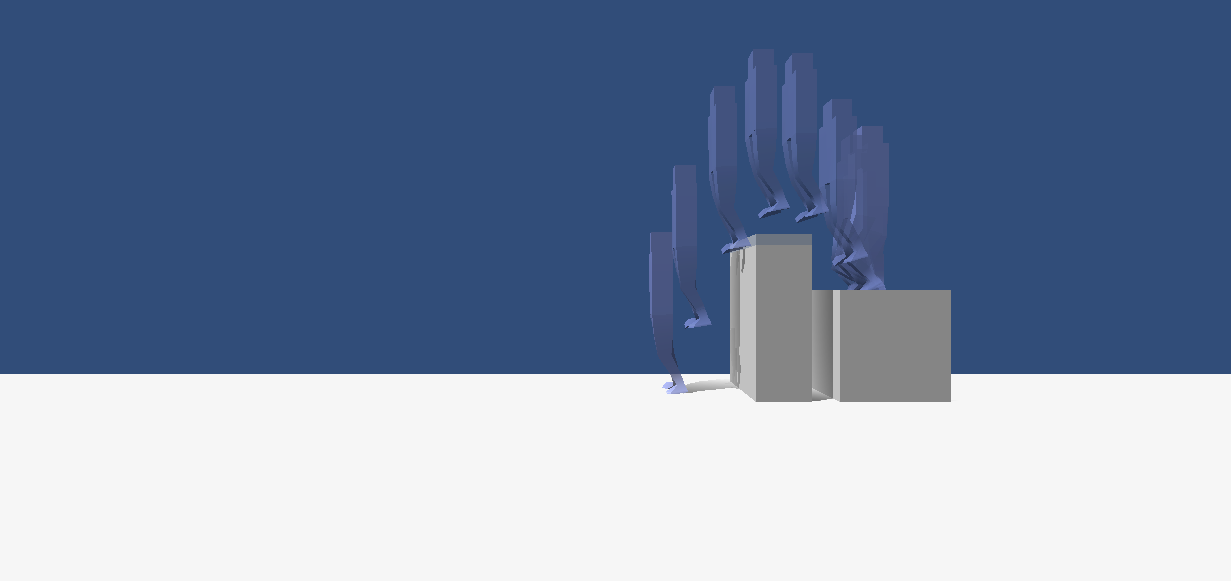
\includegraphics[width=\textwidth]{images/trials/K200000global/ComplexScene/BestPlacement/side-camera-composite.png}
	\end{subfigure}\vspace{1mm}
	%\raggedleft
	\framesubfig{images/trials/K200000global/ComplexScene/BestPlacement/side/frame0001.png}
	\framesubfig{images/trials/K200000global/ComplexScene/BestPlacement/side/frame0005.png}
	\framesubfig{images/trials/K200000global/ComplexScene/BestPlacement/side/frame0010.png}
	\framesubfig{images/trials/K200000global/ComplexScene/BestPlacement/side/frame0015.png}
	\framesubfig{images/trials/K200000global/ComplexScene/BestPlacement/side/frame0020.png}
	\framesubfig{images/trials/K200000global/ComplexScene/BestPlacement/side/frame0030.png}
	\framesubfig{images/trials/K200000global/ComplexScene/BestPlacement/side/frame0035.png}
	\framesubfig{images/trials/K200000global/ComplexScene/BestPlacement/side/frame0040.png}
	\framesubfig{images/trials/K200000global/ComplexScene/BestPlacement/side/frame0045.png}
	\framesubfig{images/trials/K200000global/ComplexScene/BestPlacement/side/frame0050.png}
	\framesubfig{images/trials/K200000global/ComplexScene/BestPlacement/side/frame0054.png}
	\caption[Animation of a jump over an obstacle]{Pictured is an animation of a complex scene, in which the character must jump from on top of a box, over another box and land on the ground.  The first image in the figure shows the frames composited into one image to visualize the full motion, while the remaining images show the individual frames.  This run used $t_{windup}=0.2s$ and $t_{air}=0.5s$.}
	\label{fig:complex_scene}
\end{figure}

\begin{table}[ht]
	\centering
	\begin{tabular}{|p{0.1\textwidth}|p{0.9\textwidth}|}
		\hline\vspace{1mm}
		1m forward &%
			\floatedfig{images/trials/K200000global/100cm/frame0001.png}
			\floatedfig{images/trials/K200000global/100cm/frame0005.png}
			\floatedfig{images/trials/K200000global/100cm/frame0010.png}
			\floatedfig{images/trials/K200000global/100cm/frame0015.png}
			\floatedfig{images/trials/K200000global/100cm/frame0020.png}
			\floatedfig{images/trials/K200000global/100cm/frame0024.png}
			\\ \hline
		1.3m forward &%
			\floatedfig{images/trials/K200000global/130cm/frame0001.png}
			\floatedfig{images/trials/K200000global/130cm/frame0005.png}
			\floatedfig{images/trials/K200000global/130cm/frame0010.png}
			\floatedfig{images/trials/K200000global/130cm/frame0015.png}
			\floatedfig{images/trials/K200000global/130cm/frame0020.png}
			\floatedfig{images/trials/K200000global/130cm/frame0024.png}
			\\ \hline
		1.6m forward &%
			\floatedfig{images/trials/K200000global/160cm/frame0001.png}
			\floatedfig{images/trials/K200000global/160cm/frame0005.png}
			\floatedfig{images/trials/K200000global/160cm/frame0010.png}
			\floatedfig{images/trials/K200000global/160cm/frame0015.png}
			\floatedfig{images/trials/K200000global/160cm/frame0020.png}
			\floatedfig{images/trials/K200000global/160cm/frame0024.png}
			\\ \hline
		1.9m forward &%
			\floatedfig{images/trials/K200000global/190cm/frame0001.png}
			\floatedfig{images/trials/K200000global/190cm/frame0005.png}
			\floatedfig{images/trials/K200000global/190cm/frame0010.png}
			\floatedfig{images/trials/K200000global/190cm/frame0015.png}
			\floatedfig{images/trials/K200000global/190cm/frame0020.png}
			\floatedfig{images/trials/K200000global/190cm/frame0025.png}
			\floatedfig{images/trials/K200000global/190cm/frame0028.png}
			\\ \hline
		0.5m box &%
			\floatedfig{images/trials/K200000global/50cmBox/frame0001.png}
			\floatedfig{images/trials/K200000global/50cmBox/frame0005.png}
			\floatedfig{images/trials/K200000global/50cmBox/frame0010.png}
			\floatedfig{images/trials/K200000global/50cmBox/frame0015.png}
			\floatedfig{images/trials/K200000global/50cmBox/frame0020.png}
			\floatedfig{images/trials/K200000global/50cmBox/frame0025.png}
			\floatedfig{images/trials/K200000global/50cmBox/frame0030.png}
			\floatedfig{images/trials/K200000global/50cmBox/frame0035.png}
			\floatedfig{images/trials/K200000global/50cmBox/frame0040.png}
			\floatedfig{images/trials/K200000global/50cmBox/frame0045.png}
			\\ \hline
		0.75m box &%
			\floatedfig{images/trials/K200000global/75cmBox/frame0001.png}
			\floatedfig{images/trials/K200000global/75cmBox/frame0005.png}
			\floatedfig{images/trials/K200000global/75cmBox/frame0010.png}
			\floatedfig{images/trials/K200000global/75cmBox/frame0015.png}
			\floatedfig{images/trials/K200000global/75cmBox/frame0020.png}
			\floatedfig{images/trials/K200000global/75cmBox/frame0025.png}
			\floatedfig{images/trials/K200000global/75cmBox/frame0030.png}
			\floatedfig{images/trials/K200000global/75cmBox/frame0035.png}
			\floatedfig{images/trials/K200000global/75cmBox/frame0039.png}
			\\ \hline
	\end{tabular}
	\caption[Table of frame sequences for forward and box jumps, $k=20000$ global]{Table of forward and box jump motions for a character with global $k=20000$, $t_{windup}=0.2s$, and $t_{air} = 0.5s$.  The boxes were placed 0.75m in front of the character, with the character's target destination set 0.3m in front of the character on top of the box.}
    \label{tab:forward_200k_g}
\end{table}

\begin{table}[ht]
	\centering
	\begin{tabular}{|p{0.1\textwidth}|p{0.9\textwidth}|}
		\hline\vspace{1mm}
		1m right &%
			\floatedfig{images/trials/K200000global/100cmRight/front/frame0001.png}
			\floatedfig{images/trials/K200000global/100cmRight/front/frame0005.png}
			\floatedfig{images/trials/K200000global/100cmRight/front/frame0010.png}
			\floatedfig{images/trials/K200000global/100cmRight/front/frame0015.png}
			\floatedfig{images/trials/K200000global/100cmRight/front/frame0020.png}
			\floatedfig{images/trials/K200000global/100cmRight/front/frame0025.png}
			\floatedfig{images/trials/K200000global/100cmRight/front/frame0030.png}
			\floatedfig{images/trials/K200000global/100cmRight/front/frame0035.png}
			\floatedfig{images/trials/K200000global/100cmRight/front/frame0040.png}
			\\ \hline
		1.3m right &%
			\floatedfig{images/trials/K200000global/130cmRight/front/frame0041.png}
			\floatedfig{images/trials/K200000global/130cmRight/front/frame0045.png}
			\floatedfig{images/trials/K200000global/130cmRight/front/frame0050.png}
			\floatedfig{images/trials/K200000global/130cmRight/front/frame0055.png}
			\floatedfig{images/trials/K200000global/130cmRight/front/frame0060.png}
			\floatedfig{images/trials/K200000global/130cmRight/front/frame0065.png}
			\floatedfig{images/trials/K200000global/130cmRight/front/frame0070.png}
			\floatedfig{images/trials/K200000global/130cmRight/front/frame0075.png}
			\floatedfig{images/trials/K200000global/130cmRight/front/frame0077.png}
			\\ \hline
		1.6m right &%
			\floatedfig{images/trials/K200000global/160cmRight/front/frame0078.png}
			\floatedfig{images/trials/K200000global/160cmRight/front/frame0083.png}
			\floatedfig{images/trials/K200000global/160cmRight/front/frame0088.png}
			\floatedfig{images/trials/K200000global/160cmRight/front/frame0093.png}
			\floatedfig{images/trials/K200000global/160cmRight/front/frame0098.png}
			\floatedfig{images/trials/K200000global/160cmRight/front/frame0103.png}
			\floatedfig{images/trials/K200000global/160cmRight/front/frame0108.png}
			\floatedfig{images/trials/K200000global/160cmRight/front/frame0111.png}
			\\ \hline
	\end{tabular}
	\caption[Table of frame sequences for sideways jumps, $k=20000$ global]{Table of right jump motions for a character with global $k=20000$, $t_{windup}=0.2s$, and $t_{air} = 0.5s$.  The target was placed at the distance listed in the table in the direction $(1, 0, 0)$ relative to the character.}
    \label{tab:side_200k_g}
\end{table}

\begin{table}[ht]
	\centering
	\begin{tabular}{|p{0.1\textwidth}|p{0.9\textwidth}|}
		\hline\vspace{1mm}
		1m forward &%
			\floatedfig{images/trials/K200000varying/100cm/frame0001.png}
			\floatedfig{images/trials/K200000varying/100cm/frame0005.png}
			\floatedfig{images/trials/K200000varying/100cm/frame0010.png}
			\floatedfig{images/trials/K200000varying/100cm/frame0015.png}
			\floatedfig{images/trials/K200000varying/100cm/frame0020.png}
			\floatedfig{images/trials/K200000varying/100cm/frame0024.png}
			\\ \hline
		1.3m forward &%
			\floatedfig{images/trials/K200000varying/130cm/frame0001.png}
			\floatedfig{images/trials/K200000varying/130cm/frame0005.png}
			\floatedfig{images/trials/K200000varying/130cm/frame0010.png}
			\floatedfig{images/trials/K200000varying/130cm/frame0015.png}
			\floatedfig{images/trials/K200000varying/130cm/frame0020.png}
			\floatedfig{images/trials/K200000varying/130cm/frame0024.png}
			\\ \hline
		1.6m forward &%
			\floatedfig{images/trials/K200000varying/160cm/frame0001.png}
			\floatedfig{images/trials/K200000varying/160cm/frame0005.png}
			\floatedfig{images/trials/K200000varying/160cm/frame0010.png}
			\floatedfig{images/trials/K200000varying/160cm/frame0015.png}
			\floatedfig{images/trials/K200000varying/160cm/frame0020.png}
			\floatedfig{images/trials/K200000varying/160cm/frame0024.png}
			\\ \hline
		1.9m forward &%
			\floatedfig{images/trials/K200000varying/190cm/frame0001.png}
			\floatedfig{images/trials/K200000varying/190cm/frame0005.png}
			\floatedfig{images/trials/K200000varying/190cm/frame0010.png}
			\floatedfig{images/trials/K200000varying/190cm/frame0015.png}
			\floatedfig{images/trials/K200000varying/190cm/frame0020.png}
			\floatedfig{images/trials/K200000varying/190cm/frame0025.png}
			\floatedfig{images/trials/K200000varying/190cm/frame0028.png}
			\\ \hline
		0.5m box &%
			\floatedfig{images/trials/K200000varying/50cmBox/frame0001.png}
			\floatedfig{images/trials/K200000varying/50cmBox/frame0005.png}
			\floatedfig{images/trials/K200000varying/50cmBox/frame0010.png}
			\floatedfig{images/trials/K200000varying/50cmBox/frame0015.png}
			\floatedfig{images/trials/K200000varying/50cmBox/frame0020.png}
			\floatedfig{images/trials/K200000varying/50cmBox/frame0030.png}
			\floatedfig{images/trials/K200000varying/50cmBox/frame0035.png}
			\floatedfig{images/trials/K200000varying/50cmBox/frame0040.png}
			\floatedfig{images/trials/K200000varying/50cmBox/frame0045.png}
			\floatedfig{images/trials/K200000varying/50cmBox/frame0046.png}
			\\ \hline
		0.75m box &%
			\floatedfig{images/trials/K200000varying/75cmBox/frame0001.png}
			\floatedfig{images/trials/K200000varying/75cmBox/frame0005.png}
			\floatedfig{images/trials/K200000varying/75cmBox/frame0010.png}
			\floatedfig{images/trials/K200000varying/75cmBox/frame0015.png}
			\floatedfig{images/trials/K200000varying/75cmBox/frame0025.png}
			\floatedfig{images/trials/K200000varying/75cmBox/frame0030.png}
			\floatedfig{images/trials/K200000varying/75cmBox/frame0035.png}
			\floatedfig{images/trials/K200000varying/75cmBox/frame0039.png}
			\\ \hline
	\end{tabular}
	\caption[Table of frame sequences for forward and box jumps, $k=20000$ varying]{Table of forward and box jump motions for a character with varying $k \approx 20000$, $t_{windup}=0.2s$, and $t_{air} = 0.5s$.  The boxes were placed 0.75m in front of the character, with the character's target destination set 0.3m in front of the character on top of the box.}
    \label{tab:forward_200k_v}
\end{table}

\begin{table}[ht]
	\centering
	\begin{tabular}{|p{0.1\textwidth}|p{0.9\textwidth}|}
		\hline\vspace{1mm}
		1.6m forward (global $k=20000$) &%
			\floatedfig{images/trials/K200000globaluneven/160cm/frame0001.png}
			\floatedfig{images/trials/K200000globaluneven/160cm/frame0005.png}
			\floatedfig{images/trials/K200000globaluneven/160cm/frame0010.png}
			\floatedfig{images/trials/K200000globaluneven/160cm/frame0015.png}
			\floatedfig{images/trials/K200000globaluneven/160cm/frame0020.png}
			\floatedfig{images/trials/K200000globaluneven/160cm/frame0025.png}
			\floatedfig{images/trials/K200000globaluneven/160cm/frame0030.png}
			\floatedfig{images/trials/K200000globaluneven/160cm/frame0035.png}
			\\ \hline
		1.9m forward (global $k=20000$) &%
			\floatedfig{images/trials/K200000globaluneven/190cm/frame0036.png}
			\floatedfig{images/trials/K200000globaluneven/190cm/frame0041.png}
			\floatedfig{images/trials/K200000globaluneven/190cm/frame0046.png}
			\floatedfig{images/trials/K200000globaluneven/190cm/frame0051.png}
			\floatedfig{images/trials/K200000globaluneven/190cm/frame0056.png}
			\floatedfig{images/trials/K200000globaluneven/190cm/frame0061.png}
			\floatedfig{images/trials/K200000globaluneven/190cm/frame0066.png}
			\\ \hline
		1.6m forward (varying $k=20000$) &%
			\floatedfig{images/trials/K200000varyinguneven/160cm/frame0001.png}
			\floatedfig{images/trials/K200000varyinguneven/160cm/frame0005.png}
			\floatedfig{images/trials/K200000varyinguneven/160cm/frame0010.png}
			\floatedfig{images/trials/K200000varyinguneven/160cm/frame0015.png}
			\floatedfig{images/trials/K200000varyinguneven/160cm/frame0020.png}
			\floatedfig{images/trials/K200000varyinguneven/160cm/frame0025.png}
			\floatedfig{images/trials/K200000varyinguneven/160cm/frame0030.png}
			\floatedfig{images/trials/K200000varyinguneven/160cm/frame0032.png}
			\\ \hline
		1.9m forward (varying $k=20000$) &%
			\floatedfig{images/trials/K200000varyinguneven/190cm/frame0001.png}
			\floatedfig{images/trials/K200000varyinguneven/190cm/frame0005.png}
			\floatedfig{images/trials/K200000varyinguneven/190cm/frame0010.png}
			\floatedfig{images/trials/K200000varyinguneven/190cm/frame0015.png}
			\floatedfig{images/trials/K200000varyinguneven/190cm/frame0020.png}
			\floatedfig{images/trials/K200000varyinguneven/190cm/frame0025.png}
			\floatedfig{images/trials/K200000varyinguneven/190cm/frame0030.png}
			\floatedfig{images/trials/K200000varyinguneven/190cm/frame0034.png}
			\\ \hline
	\end{tabular}
	\caption[Table of frame sequences for jumps with uneven leg strengths, $k=20000$ global]{Table of forward jumping motions with uneven muscle strengths between legs, using $t_{windup}=0.2s$ and $t_{air}=0.5s$.}
    \label{tab:forward_200k_u}
\end{table}

\begin{table}[ht]
	\label{tab:superman_forward}
	\centering
	\begin{tabular}{|p{0.1\textwidth}|p{0.9\textwidth}|}
		\hline
		1m forward &%
			\floatedfig{images/trials/k1e10global/1m/frame0001.png}
			\floatedfig{images/trials/k1e10global/1m/frame0005.png}
			\floatedfig{images/trials/k1e10global/1m/frame0011.png}
			\floatedfig{images/trials/k1e10global/1m/frame0015.png}
			\floatedfig{images/trials/k1e10global/1m/frame0020.png}
			\floatedfig{images/trials/k1e10global/1m/frame0025.png} 
			\floatedfig{images/trials/k1e10global/1m/frame0030.png}
			\floatedfig{images/trials/k1e10global/1m/frame0033.png}
			\floatedfig{images/trials/k1e10global/1m/frame0035.png}%
			\\ \hline%
		10m forward &%
			\floatedfig{images/trials/k1e10global/10m/1s1point5s/frame0042.png}
			\floatedfig{images/trials/k1e10global/10m/1s1point5s/frame0047.png}
			\floatedfig{images/trials/k1e10global/10m/1s1point5s/frame0050.png}
			\floatedfig{images/trials/k1e10global/10m/1s1point5s/frame0053.png}
			\floatedfig{images/trials/k1e10global/10m/1s1point5s/frame0055.png}
			\floatedfig{images/trials/k1e10global/10m/1s1point5s/frame0060.png}
			\floatedfig{images/trials/k1e10global/10m/1s1point5s/frame0064.png}
			\floatedfig{images/trials/k1e10global/10m/1s1point5s/frame0066.png}
			\floatedfig{images/trials/k1e10global/10m/1s1point5s/frame0070.png}
			\floatedfig{images/trials/k1e10global/10m/1s1point5s/frame0075.png}
			\floatedfig{images/trials/k1e10global/10m/1s1point5s/frame0080.png}
			\floatedfig{images/trials/k1e10global/10m/1s1point5s/frame0085.png}
			\floatedfig{images/trials/k1e10global/10m/1s1point5s/frame0090.png}
			\floatedfig{images/trials/k1e10global/10m/1s1point5s/frame0095.png}
			\floatedfig{images/trials/k1e10global/10m/1s1point5s/frame0101.png}
			\\ \hline%
	\end{tabular}
	\caption[Table of frame sequences for forward jumps, $k=1 \times 10^10$ global]{Above are generated frame sequences for the super human trial, where the $k$ values were chosen such that the character could leap over a tall building, a 100m tall box.  Animations above were generated for 1m, 10m, and 100m forward jumps.  The 100m forward jump is not pictured due to the difficulty of capture, as either the jump was out of the range of the camera or the camera was too far to clearly see the animation.}
\end{table}

\begin{table}[ht]
	\label{tab:superman_box}
	\centering
	\begin{tabular}{|p{0.1\textwidth}|p{0.9\textwidth}|}
		\hline\vspace{1mm}
		1m box &%
			\floatedfig{images/trials/k1e10global/1mBox/frame0001.png}
			\floatedfig{images/trials/k1e10global/1mBox/frame0005.png}
			\floatedfig{images/trials/k1e10global/1mBox/frame0010.png}
			\floatedfig{images/trials/k1e10global/1mBox/frame0020.png}
			\floatedfig{images/trials/k1e10global/1mBox/frame0025.png}
			\floatedfig{images/trials/k1e10global/1mBox/frame0030.png}
			\floatedfig{images/trials/k1e10global/1mBox/frame0035.png}
			\floatedfig{images/trials/k1e10global/1mBox/frame0039.png}
			\\ \hline%
		100m box &%
			\floatedfig{images/trials/k1e10global/100mBox/1s5s/frame0001.png}
			\floatedfig{images/trials/k1e10global/100mBox/1s5s/frame0005.png}
			\floatedfig{images/trials/k1e10global/100mBox/1s5s/frame0010.png}
			\floatedfig{images/trials/k1e10global/100mBox/1s5s/frame0015.png}
			\floatedfig{images/trials/k1e10global/100mBox/1s5s/frame0020.png}
			\floatedfig{images/trials/k1e10global/100mBox/1s5s/frame0025.png}
			\floatedfig{images/trials/k1e10global/100mBox/1s5s/frame0030.png}
			\floatedfig{images/trials/k1e10global/100mBox/1s5s/frame0035.png}
			\floatedfig{images/trials/k1e10global/100mBox/1s5s/frame0040.png}
			\floatedfig{images/trials/k1e10global/100mBox/1s5s/frame0045.png}
			\floatedfig{images/trials/k1e10global/100mBox/1s5s/frame0050.png}
			\floatedfig{images/trials/k1e10global/100mBox/1s5s/frame0055.png}
			\floatedfig{images/trials/k1e10global/100mBox/1s5s/frame0060.png}
			\floatedfig{images/trials/k1e10global/100mBox/1s5s/frame0065.png}
			\floatedfig{images/trials/k1e10global/100mBox/1s5s/frame0070.png}
			\floatedfig{images/trials/k1e10global/100mBox/1s5s/frame0075.png}
			\floatedfig{images/trials/k1e10global/100mBox/1s5s/frame0080.png}
			\floatedfig{images/trials/k1e10global/100mBox/1s5s/frame0085.png}
			\floatedfig{images/trials/k1e10global/100mBox/1s5s/frame0090.png}
			\floatedfig{images/trials/k1e10global/100mBox/1s5s/frame0095.png}
			\floatedfig{images/trials/k1e10global/100mBox/1s5s/frame0100.png}
			\floatedfig{images/trials/k1e10global/100mBox/1s5s/frame0105.png}
			\floatedfig{images/trials/k1e10global/100mBox/1s5s/frame0110.png}
			\floatedfig{images/trials/k1e10global/100mBox/1s5s/frame0115.png}
			\floatedfig{images/trials/k1e10global/100mBox/1s5s/frame0120.png}
			\floatedfig{images/trials/k1e10global/100mBox/1s5s/frame0125.png}
			\floatedfig{images/trials/k1e10global/100mBox/1s5s/frame0130.png}
			\floatedfig{images/trials/k1e10global/100mBox/1s5s/frame0135.png}
			\floatedfig{images/trials/k1e10global/100mBox/1s5s/frame0140.png}
			\floatedfig{images/trials/k1e10global/100mBox/1s5s/frame0145.png}
			\floatedfig{images/trials/k1e10global/100mBox/1s5s/frame0148.png}
			\\ \hline
	\end{tabular}
	\caption[Table of frame sequences for box jumps, $k=1 \times 10^10$ global]{Animations of 1m and 100m box jumps for the super human.  This run uses $t_{windup} = 1s$ and $t_{air} = 5s$.}
\end{table}

\section{Limitations}
\label{section:limitations}
Our system has a number of limitations and failure cases.  First is that there are many constants to be specified, which is work intensive but gives freedom to make wide changes to the animation by tuning parameters

There are numerous small issues with the calculations caused by strange or unexpected interactions.  Foremost is the behavior of rotations and angle measurement in \unity{}.  Angles are read and interacted with as Euler angles, pitch, roll, and yaw, or rotation about the x, z, and y axes respectively.  Rotations, however, are stored and calculated by the engine in the form of quaternions in order to avoid gimbal lock and allow smoother interpolation between rotations.  Due to the conversions between the two, and various manipulations that occur in the scene, this can result in angles not restricted to $[-360, 360]$ degrees, and can result in jumps between positive and negative angles.  A solution would be to restrict the angles to positive angles in the range $[0,360]$ for all calculations and manipulations, but this makes specifying constraints more complex.  

Problems with angle also arise as the angle of the joint does not necessarily reflect the angle between the bones.  For example, when the knee is fully extended, the joint angle stored in the object is 0, but the angle between the bones is $\pi$ radians.  A solution is to calculate the angle between the bones of the joint when needed using the dot product of the vectors between the joint and its parent and the joint and its child.  We did not realize that there was still an issue with angle specification as the issue was balanced out as the supplementary angle was used erroneously, but a fully correct implementation would be desirable for true consistency.  The data was collected with the flawed implementation, though as previously stated it produced similar results.

Movement of the upper body is very minimal, and is quite unlike a human performing a long jump.  This is likely due to the restriction of pelvis reposition to the region over the supporting polygon.  Humans frequently move their pelvises far behind their supporting polygon, compensating using the weight of their upper body.  The usage of rapid movement of the upper body to aid in acceleration is also a factor we do not consider, such as the effects of arm swing on a jump.

As our simulation was focused on the movements leading to the airborne phase, the handling of in air maneuvers and landing are overly simplistic.  After the character becomes airborne, the pelvis will generally be displaced in the direction of acceleration relative to the feet.  The character should maneuver while airborne such that their feet are in front of their body to prepare for landing.  For landing, a reverse of the windup for the energy simulation could be used, loading the muscles in the legs to offset the kinetic energy the character has from the jump, converting it to elastic energy in the muscles.  Landing and airborne phases should be handled ideally by a separate controller.

Our inverse kinematic solver is also very simple, and brings its own issues due to this simplicity.  This algorithm was chosen specifically to minimize time, effort, and resources spent on the inverse kinematic component, in favor of the simulation itself.  With a different inverse kinematic solver, better results could be achieved.

The output of our simulation is currently image frames as well as the direct visualization through \unity{}, as opposed to a key frame animation in a format such as FBX, which could be utilized in video games.  An \maya{}  plugin that runs our simulation would also be more useful for allowing creation of animations if a real-time frame rate cannot be achieved.

\section{Summary}
\label{section:results_summary}
Plausible animations were created, with empirically determined $k$ values around 20000.  Analysis shows different values would be theoretically more realistic, but the empirically determined values still produced reasonable animations.  Animations were produced for a normal strength human as well as a super human for forward standing jumps, sideways standing jumps, and box jumps.  A scene was constructed in which the character jumped from on top of a box, over an obstacle, and landed on the ground below to show a more complex scene.  We discussed in this chapter the values used and method for collecting data, and presented sets of frames collected from several simulations with a variety of scenes.  Animations depicted forward, sideways, and box jumps for a normal human range of strength and for a super human strength.  An animation of a character jumping over an obstacle was also presented.

%%%%%%%%%%%%%%%%%%%%%%%%%%%%%%%%%%%%%%%%%%%%%%%%%%%%%%%%%%%%%%%%%%% 
%                                                                 %
%                           FUTUREWORK                            %
%                                                                 %
%%%%%%%%%%%%%%%%%%%%%%%%%%%%%%%%%%%%%%%%%%%%%%%%%%%%%%%%%%%%%%%%%%% 
 
% \specialhead{FUTUREWORK}
\chapter{FUTURE WORK AND CONCLUSION}
\label{chapter:future_work}
In this chapter we discuss future work and conclude our discussion of research on this simulation.  Section \ref{section:future_work} discusses possible and planned work on this topic, as well as potential future work in this and closely related lines of study.  Section \ref{section:conclusion} concludes this document with final thoughts and a summary of the document.

\section{Future Work}
\label{section:future_work}

We planned some further work that we decided was beyond the scope of this thesis.  Our current system does not allow much flexibility with specification of the path the character travels for its jump.  Jumping path estimation could be performed based on a policy.  Possible policies are achieving a height while jumping to a target destination, pathing to clear an object or intersect with an object, follow a path defined by the user, and jumping with a user specified velocity or speed.  These policies would require a smarter handling of the in air phase of the jump, which would be best implemented as a secondary controller to allow controller composition for more complex motions.  A more complex in air controller would ideally handle cases such as acrobatics, in air maneuvers, and checking for and handling collisions.

Current work exists for landing motions such as described in chapter \ref{chapter:previous_work}.   \liufall{} describes an example of one such controller for a falling and landing motions.  Incorporation of such other controllers would allow creation of more complex animations.  A separate controller could also be used for improving the motions of the upper body for each of these phases.  This could be used to create complex freerunning animations such as vaults and wall runs which are becoming prevalent in video games such as Mirror's Edge.

To help with choosing values, a learning model could be applied.  Animations could be marked as successful and desirable by humans to train an algorithm to choose desirable constants for the muscles given target destinations.  Machine learning could also be applied for learning a function to determine muscle load in the windup phase of our simulation.  Intuitively the situation seems to fit a learning model well, but more study would be required.

Both simulations were solved using a sampling solution, but could have been solved using an optimization problem.  Solving the optimization problem, such as the quadratic program in \ref{subsection:energy_prob} would likely provide a better solution and would give stronger guarantees of optimality.  This would likely decrease performance.

Our animation output is currently images.  A more desirable animation output would be key frames storing the positions and orientations for each joint of the character's skeleton, which could then be used in a game or video as a pre-baked animation.  An implementation as a plugin for \maya{} could also be more desirable, as it could then be incorporated into an artist's work flow.  We chose not to use \maya{} initially for an implementation initially due to familiarity with \unity{} and so that we could obtain live visuals of the simulation with debugging information easily as the simulation was performed and animation played.

Another option would be to utilize MecAnim, a feature of \unity{}.  We chose not to use this feature while performing the initial research, due to lack of understanding of the limitations and features available in MecAnim.  After completing further research, there are many components of MecAnim that would improve our simulation and increase its ease of incorporation into game development and animation workflows.  Our simulation could be re-tooled to output animation clips for MecAnim, and our constraint system replaced with the one provided by MecAnim.  MecAnim muscles do not provide the functionality required, so our muscle component would need to be modified and reapplied to the skeleton.  As is, our simulation is very close to producing output that could be used as an input to MecAnim, making this a promising direction for future work on the implementation.

\section{Conclusion and Summary}
\label{section:conclusion}

In this thesis, we discussed the need for a more efficient way to produce character animations for video games and film.  We then presented a simulation based approach for creating such animations for a jumping motion of a character to reach a given target position.  Our system used two different types of simulation: torque based and energy based.  The torque based simulation failed to produce good results, but we collected frame data for a variety of situations using the energy based simulation.  We then described our methods for visualizing the animations to quantify and qualify the performance, giving visual information in an animated format and still format.


\specialhead{References}

\bibliography{IEEEabrv,research}
\bibliographystyle{ieeetran}
% \include{Bibliography} 	% bibliography
%\include{rpiapp} 	% appendix
\end{document}
